\documentclass[11pt,titlepage]{article}
\usepackage[centertags]{amsmath}
\usepackage{hyperref}
\usepackage{url}
\usepackage{amsfonts}
\usepackage{amssymb}
\usepackage{latexsym}
\usepackage{pdfpages}
\usepackage{amsthm}
\usepackage{newlfont}
\usepackage{graphicx}
\usepackage[subrefformat=parens, labelformat=parens]{subfig}
\usepackage{listings}
\usepackage{booktabs}
\usepackage{abstract}
\usepackage{tikz}
\usepackage{caption}
%\usepackage{subcaption}
\usepackage{algorithm,algorithmic}
\usepackage[]{mcode}
\bibliographystyle{amsplain}
\renewcommand{\textfraction}{0.15}
\renewcommand{\topfraction}{0.85}
\renewcommand{\bottomfraction}{0.65}
\renewcommand{\floatpagefraction}{0.60}
%\newcommand{\topfigrule}{%
%  \vspace*{5pt}\hrule\vspace{-5.4pt}}
%\newcommand{\botfigrule}{\vspace*{-5.4pt}\hrule\vspace{5pt}}


\newlength{\defbaselineskip}
\setlength{\defbaselineskip}{\baselineskip}
\newcommand{\setlinespacing}[1]%
           {\setlength{\baselineskip}{#1 \defbaselineskip}}
\newcommand{\doublespacing}{\setlength{\baselineskip}%
                           {2.0 \defbaselineskip}}
\newcommand{\singlespacing}{\setlength{\baselineskip}{\defbaselineskip}}
% MATH -------------------------------------------------------------------
\newcommand{\A}{{\cal A}}
\newcommand{\h}{{\cal H}}
\newcommand{\s}{{\cal S}}
\newcommand{\W}{{\cal W}}
\newcommand{\D}{{\cal D}}
\newcommand{\NN}{\mathbb N}
\newcommand{\BH}{\mathbf B(\cal H)}
\newcommand{\KH}{\cal  K(\cal H)}
\newcommand{\Int}{\mathbb Z}
\newcommand{\Complex}{\mathbb C}
\newcommand{\Field}{\mathbb F}
\newcommand{\RPlus}{[0,\infty)}
\newcommand{\rip}{\operatorname{RIP}}
\newcommand{\pj}{\text{Proj}}
\newcommand{\csp}{\overline{\operatorname{span}}}
\newcommand{\spn}{\operatorname{span}}
%
\newcommand{\norm}[1]{\left\Vert#1\right\Vert}
\newcommand{\essnorm}[1]{\norm{#1}_{\text{\rm\normalshape ess}}}
\newcommand{\abs}[1]{\left\vert#1\right\vert}
\newcommand{\set}[1]{\left\{#1\right\}}
\newcommand{\seq}[1]{\left<#1\right>}
\newcommand{\eps}{\varepsilon}
\newcommand{\To}{\longrightarrow}
\newcommand{\RE}{\operatorname{Re}}
\newcommand{\IM}{\operatorname{Im}}
\newcommand{\supp}{\text{supp}}
\newcommand{\Poly}{{\cal{P}}(E)}
\newcommand{\EssD}{{\cal{D}}}
\newcommand{\argmin}{\operatornamewithlimits{argmin}}
\newcommand{\argmax}{\operatornamewithlimits{argmax}}
\newcommand{\Fc}{\mathcal{F}}
\newcommand{\Ac}{\mathcal{A}}
\newcommand{\Ic}{\mathcal{I}}
\newcommand{\Nc}{\mathcal{N}}
\newcommand{\Ex}{\mathbb{E}}
\newcommand{\real}{\mathbb{R}}
%\newcommand{\Pr}{\textsc{P}}
\newcommand{\cL}{\mathcal{L}}
\newcommand{\cF}{\mathcal{F}}
\newcommand{\Xf}{\mathfrak{X}}
\newcommand{\bx}{\boldsymbol{x}}
\newcommand{\by}{\boldsymbol{y}}
\newcommand{\bw}{\boldsymbol{w}}
\newcommand{\bmu}{\boldsymbol{\mu}}
\newcommand{\bthe}{\boldsymbol{\theta}}
\newcommand{\bA}{\boldsymbol{A}}
\newcommand{\ba}{\boldsymbol{a}}
\newcommand{\bb}{\boldsymbol{b}}
\newcommand{\bd}{\boldsymbol{d}}
\newcommand{\bff}{\boldsymbol{f}}
\newcommand{\bF}{\boldsymbol{F}}
\newcommand{\bp}{\boldsymbol{p}}
\newcommand{\bG}{\boldsymbol{G}}
\newcommand{\bg}{\boldsymbol{g}}
\newcommand{\bh}{\boldsymbol{h}}
\newcommand{\bH}{\boldsymbol{H}}
\newcommand{\bk}{\boldsymbol{k}}
\newcommand{\bL}{\boldsymbol{L}}
\newcommand{\bs}{\boldsymbol{s}}
\newcommand{\bm}{\boldsymbol{m}}
\newcommand{\bn}{\boldsymbol{n}}
\newcommand{\bP}{\boldsymbol{P}}
\newcommand{\bR}{\boldsymbol{R}}
\newcommand{\bI}{\boldsymbol{I}}
\newcommand{\bJ}{\boldsymbol{J}}
\newcommand{\bQ}{\boldsymbol{Q}}
\newcommand{\bU}{\boldsymbol{U}}
\newcommand{\bV}{\boldsymbol{V}}
\newcommand{\bLam}{\boldsymbol{\Lambda}}
\newcommand{\bzero}{\boldsymbol{0}}
\newcommand{\diag}{\mathrm{diag}}
\newcommand{\mymatrix}[1]{\begin{bmatrix} #1\end{bmatrix}}
\newcommand{\comment}[1]{}
\newcommand{\tr}{{\text{tr}}}
\newcommand{\hx}{\hat{\mathbf{x}}}
\newcommand{\hy}{\hat{\mathbf{y}}}
\newcommand{\hz}{\hat{\mathbf{z}}}
\newcommand{\sff}{\mathsf{f}}





% THEOREMS ---------------------------------------------------------------
\theoremstyle{plain}
\newtheorem{thm}{Theorem}[section]
\newtheorem{cor}[thm]{Corollary}
\newtheorem{lem}{Lemma}[section]
\newtheorem{prop}[thm]{Proposition}
%
\theoremstyle{definition}
\newtheorem{defn}{Definition}[section]
\newtheorem{eg}{Example}[section]
%
\theoremstyle{remark}
\newtheorem{rem}{Remark}[section]
%
\numberwithin{equation}{section}
\renewcommand{\theequation}{\thesection.\arabic{equation}}
\newcommand{\ds}{\displaystyle}
\newtheorem{assum}{Assumption}
\newtheorem{them}{Theorem}[section]
\newtheorem{coro}{Corollary}[section]
\setcounter{section}{-1}

\begin{document}
%\title{User Guide of Seismic Simulation, Survey, and Imaging (S3I)}
%\author{Lingchen Zhu\thanks{ 
%E-mail: lczhu@gatech.edu} , \, Entao Liu\thanks{E-mail: entao.liu@ece.gatech.edu} \, and Lijun Zhu\thanks{E-mail: lijun.zhu@gatech.edu}} \maketitle
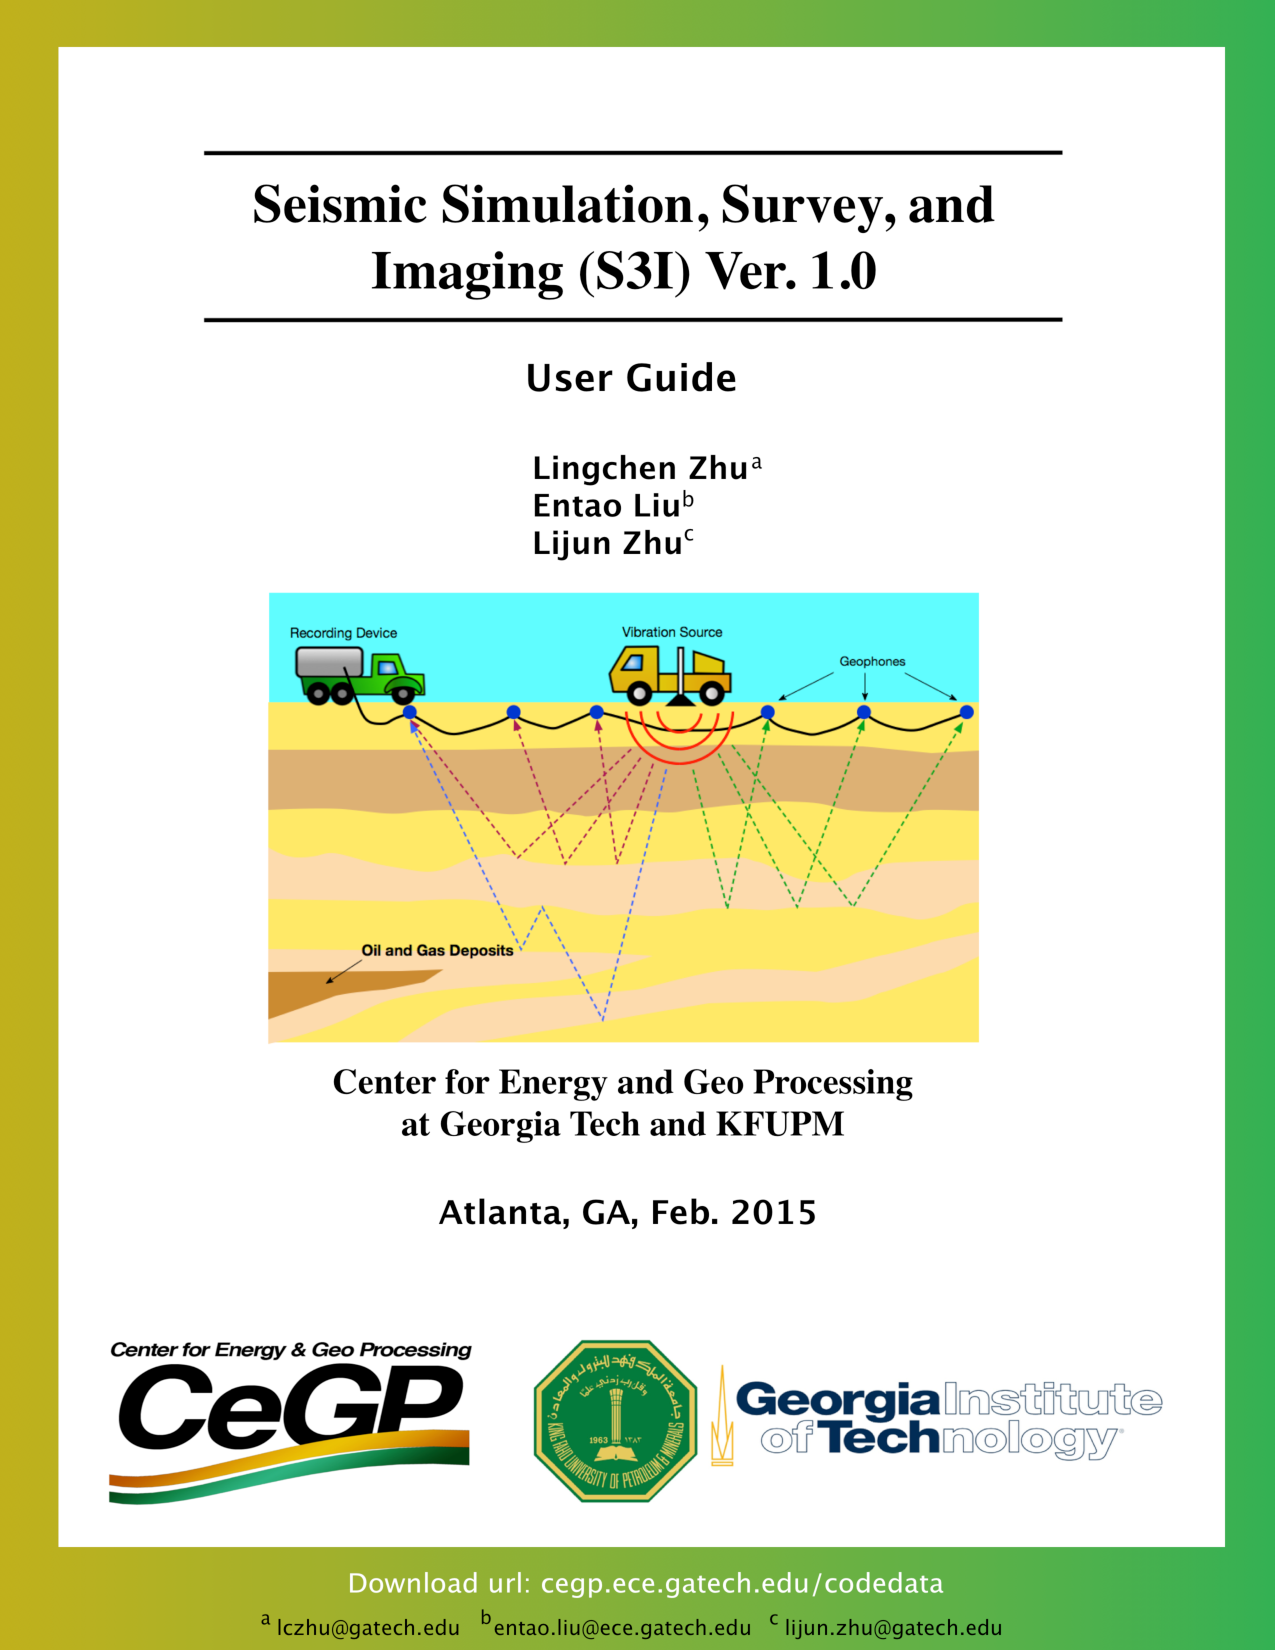
\includepdf[pages={1}]{Fig/titlepage.pdf}
\tableofcontents
\newpage



\section{Requirements and License}
The S3I is a MATLAB\textsuperscript{\textregistered} based package. Besides MATLAB (2012a or later version recommend), you may also need a C++ compiler (e.g. gcc or Microsoft C/C++ compiler) to generate the MEX-files if none of the provided MEX-files is compatible with your system architecture. In order to run parallel computing, MPI is also required and here we recommend OpenMPI.

S3I is a free software package: you can redistribute it and/or modify it under the terms of the GNU General Public License as published by the Free Software Foundation, version 2.0 of the License only. This S3I package is distributed in the hope that it will be useful, but WITHOUT ANY WARRANTY. If you find any glitches or bugs within it, please contact the authors. We appreciate your contributions. 



\section{Introduction}
The S3I is designed to provide a package for numerical simulations in exploration geophysics. It targets students as well as professionals in exploration geophysics. The most important purpose is to provide an easy, well organized library to the interested users to learn some popular algorithms and numerical schemes in exploration geophysics rather than the high performance of the computation. Thus, MATLAB is adopted as the coding platform for the readability of the code, ease of data visualization, etc. It is well known that nested for-loops in MATLAB is much slower than the complied languages. In order to make the S3I efficient, we use C to generate MEX-files for some frequently invoked functions. Currently, the major functions have been implemented in S3I are as follows:
\begin{itemize}
\item Acoustic wave simulation for 2D/3D
\item Elastic wave simulation for 2D
\item Kirchhoff's migration
\item Reverse Time Migration (RTM)
\item Least Square RTM
\item Full Waveform Inversion (FWI)
\end{itemize}

With this user guide, the user may easily and quickly start using the S3I for appropriate applications. An exhaustive review of numerical simulation of wave equation and seismic imaging is out of the scope of this user guide. Therefore, only necessary equations are showed and explained to keep the contents concise. The Interested user is referred to the references for more details.  



\section{Numerical Simulation of Acoustic Wave}


\subsection{Acoustics Wave Equation}
The seismic method is one of the primary tools in exploration geophysics. In a seismic survey, man-made vibration sources (e.g. dynamite, viborseis trucks, and air guns) are fired off. Then the wave propagates through the subsurface geological media. The wave filed which contains direct wave, reflection, and refraction, will be recorded by the array of receivers (e.g. geophones and hydrophones). In order to simulate this physical process with computers, it is crucial to solve wave equations accurately and efficiently with numerical methods. The real earth is an elastic media, such that the seismic waves contain both P-wave and S-wave components. For simplicity, we sometimes only consider the P-wave field, which is described by an acoustic wave equation. It is verified by borehole data that the media density variations are not the main source of reflected waves \cite{Hood:1981aa}. Therefore, we usually assume a constant density of the media. Then the acoustic wave equation can be written as
\begin{equation}\label{eq:aw}
\frac{1}{v^2(\bx)}\frac{\partial^2 p(\bx, t)}{\partial t^2} + f(\bx, t) = \nabla^2 p(\bx, t),
\end{equation}
where $p(\bx)$ is the filed of pressure variation and $\bx=(z,x)$ or $\bx=(z,x,y)$ is the coordinates in the Cartesian coordinate system for the 2D and 3D case, respectively. Following the convention in geophysics, the $z$ direction is pointing downwards. The $v(\bx)$ is the velocity of P-wave at location $\bx$ and $f(\bx,t)$ is the source time function. Moreover, $\Delta$ in \eqref{eq:aw} is the Laplace operator defined as 
\begin{equation}
\Delta: =\left\{
\begin{aligned}
\frac{\partial^2}{\partial x^2}+\frac{\partial^2}{\partial z^2}~~~~~~~ & ~~~~\text{for 2D }\\
\frac{\partial^2}{\partial x^2}+\frac{\partial^2}{\partial y^2}+\frac{\partial^2}{\partial z^2} &~~~~ \text{for 3D}
\end{aligned}
\right.  
\end{equation}

The Ricker wavelet is widely used for seismic source time function whose amplitude $A(t)$ with the peak frequency $\sff$ at time $t$ is computed as:
\begin{equation}
A(t)=(1-2\pi^2 \sff^2 t^2)e^{-\pi^2 \sff^2 t^2}.
\end{equation}
The \path{src/ricker.m} provides a Ricker wavelet generator which requires the peak frequency $\sff$, number of time samples $n$, sampling interval $dt$, and peak location $t_0$ as inputs. The Figure \ref{fig:ricker} illustrates the waveform of a Ricker wavelet with peak frequency equals 20 Hz. In the S3I the user can choose from several different wavelets for the source time function (Ricker wavelet, Fuchs-Mueller wavelet, sine cube wavelet, etc) which can be generated using \path{src/waveletGenerator.m}.

\begin{figure}[htbp]
\centering
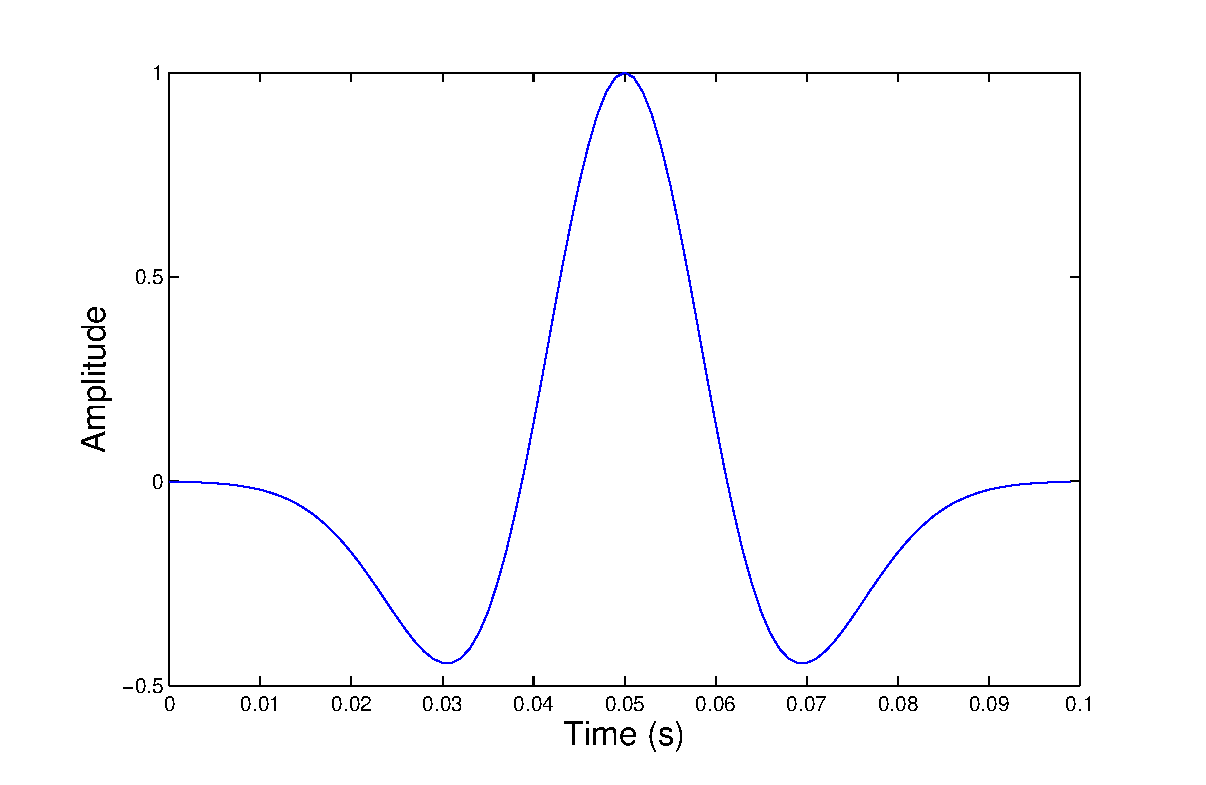
\includegraphics[width=0.8\textwidth]{Fig/ricker}
\caption{Ricker wavelet with peak frequency $\sff=20$Hz}
\label{fig:ricker}
\end{figure}


\subsection{Finite Difference Method on Standard Grid}
Currently, there are several popular methods to solve the wave equation numerically, such as pseudo-spectral method, Finite Difference Method (FDM), Finite Elements Method (FEM) method, etc. Each method has its pros and cons. Concretely, the pseudo-spectral method, which is based on Fourier transform in spatial domain, provides accurate and efficient solutions for the smoothly varied media but not for sharply varied media \cite{Kreiss:1972aa,Fornberg:1975aa,Fornberg:1987aa}. The FDM \cite{Alford:1974aa,Dablain:1986aa} adopted by S3I is widely used for its ease to implement, high accuracy, and efficiency. However, the FDM is incapable to provide accurate solution for media with complex geometry structure and rugged topography. The FEM usually provides more accurate results than FDM with a higher computational and storage expense \cite{Kurt:1984aa}. 

In order to solve the wave equation with FDM, the continuous functions and models are represented by their values at grid points and and derivatives are approximated by linear combination of these values. For instance, in a 2D region we use the uniformly distributed grid points $(z_i)_{0\le i \le I-1 }$, $(x_j)_{0\le j \le J-1}$, and $(t_n)_{0\le n \le N-1}$ given by $z_i = i\Delta z$, $x_j = j\Delta x$ and $t_n=n\Delta t$. Instead of solving the wave equation in a continuous domain (both in space and time) analytically, the FDM provides an approximated solution on these grid points.  

The estimation of derivatives in \eqref{eq:aw} is crucial in FDM. Let us revisit with the definition of the partial derivative, 
 \begin{equation}
  \begin{aligned}
  \frac{\partial p(z, x, t)}{\partial z} &= \lim\limits_{\Delta z \rightarrow 0} \frac{p(z+\Delta z, x, t) - p(z, x, t)}{\Delta z}\\
  &\approx \frac{p(z+\Delta z, x, t) - p(z, x, t)}{\Delta z}.
  \end{aligned}
  \end{equation}
Assuming the grid spacing $\Delta z$ is small enough, $(p(z+\Delta z, x, t) - p(z, x, t))/\Delta z$ is an accurate estimation of the derivative. After applying this approximation twice, we derive an central difference scheme for the second-order derivative in \eqref{eq:aw}
  \begin{equation}
  \begin{aligned}
  &\frac{\partial^2 p(z, x, t)}{\partial z^2} = \frac{\partial}{\partial z}\frac{\partial p(z, x, t)}{\partial z} \approx \frac{\frac{\partial p(z, x, t)}{\partial z} - \frac{\partial p(z-\Delta z, x, t)}{\partial z}}{\Delta z}\\
  &\approx \frac{p(z+\Delta z, x, t) - 2p(z, x, t) + p(z-\Delta z, x, t)}{\Delta z^2}.
  \end{aligned}
  \end{equation}
  
For simplicity of notation, $p_{i,j}^{(n)}:=  p(i\Delta z, j\Delta x, n\Delta t)$, $f_{i,j}^{(n)} := f(i\Delta z, j\Delta x, n\Delta t)$, $v_{i,j} := v(i\Delta z, j\Delta x)$. Therefore, a finite difference expression of 2D acoustic wave equation can be written as 
  \begin{equation}
    \begin{aligned}
    &\frac{1}{v_{i,j}^2}\frac{p_{i,j}^{(n+1)} - 2p_{i,j}^{(n)} + p_{i,j}^{(n-1)}}{\Delta t^2} - f_{i,j}^{(n)}\\
    &= \frac{p_{i+1,j}^{(n)} - 2p_{i,j}^{(n)} + p_{i-1,j}^{(n)}}{\Delta z^2} + \frac{p_{i,j+1}^{(n)} - 2p_{i,j}^{(n)} + p_{i,j-1}^{(n)}}{\Delta x^2}.
    \end{aligned}
  \end{equation}
Simple algebraic manipulations lead to a recursive expression of the wave equation,
  \begin{equation}
  \label{eq:stagGrid}
    \begin{aligned}
    &p_{i,j}^{(n+1)} = \frac{v_{i,j}^2\Delta t^2}{\Delta z^2}\left(p_{i+1,j}^{(n)} - 2p_{i,j}^{(n)} + p_{i-1,j}^{(n)}\right)\\
    &+ \frac{v_{i,j}^2\Delta t^2}{\Delta x^2}\left(p_{i,j+1}^{(n)} - 2p_{i,j}^{(n)} + p_{i,j-1}^{(n)}\right)\\
    &+ 2p_{i,j}^{(n)}-p_{i,j}^{(n-1)} + v_{i,j}^2\Delta t^2 f_{i,j}^{(n)}.
    \end{aligned}
  \end{equation}
  In \eqref{eq:stagGrid}, all values of $p$ are computed on integer grid points as illustrated in Figure \subref*{fig:stanG}. The FDM on standard grid is an easy-to-understand numerical scheme, which serves as an excellent explanatory example. However, the S3I applied another scheme, which will discuss momentarily, for its better accuracy.  
  
\begin{figure}[htbp]
\centering
  \subfloat[Standard Grid]
  {
    \begin{minipage}{0.45\linewidth}
      \begin{tikzpicture}[scale=0.85, every node/.style={scale=0.85}]
      \begin{scope}[>=latex]
      \end{scope}
      \node at (0,0)[draw,shape=circle,fill=blue,label=315:${(i,j)}$] (p0){};
      \node at (0,3)[draw,shape=circle,fill=blue,label=right:${(i-1,j)}$] (p1){};
      \node at (0,-3)[draw,shape=circle,fill=blue,label=right:${(i+1,j)}$](p2){};
      \node at (3,0)[draw,shape=circle,fill=blue,label=above:${(i,j+1)}$] (p3){};
      \node at (-3,0)[draw,shape=circle,fill=blue,label=above:${(i,j-1)}$](p4){};
      \draw (p2) -- (p0) -- (p1);
      \draw (p4) -- (p0) -- (p3);
      \end{tikzpicture}
    \end{minipage}
    \label{fig:stanG}
  }
  \hspace{1em}
  \subfloat[Staggerd Grid]
  {
    \begin{minipage}{0.45\linewidth}
      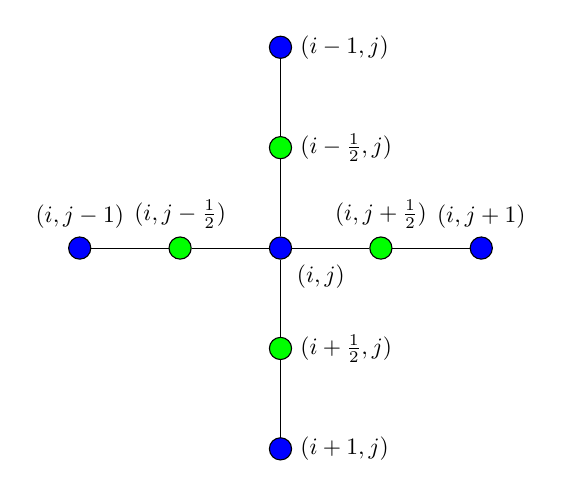
\begin{tikzpicture}[scale=0.85, every node/.style={scale=0.85}]
      \begin{scope}[>=latex]
      \end{scope}
      \node at (0,0)[draw,shape=circle,fill=blue,label=315:${(i,j)}$] (p0){};
      \node at (0,3)[draw,shape=circle,fill=blue,label=right:${(i-1,j)}$] (p1){};
      \node at (0,-3)[draw,shape=circle,fill=blue,label=right:${(i+1,j)}$](p2){};
      \node at (3,0)[draw,shape=circle,fill=blue,label=above:${(i,j+1)}$] (p3){};
      \node at (-3,0)[draw,shape=circle,fill=blue,label=above:${(i,j-1)}$](p4){};
      \node at (0,1.5)[draw,shape=circle,fill=green,label=right:${(i-\frac{1}{2},j)}$] (p5){};
      \node at (0,-1.5)[draw,shape=circle,fill=green,label=right:${(i+\frac{1}{2},j)}$](p6){};
      \node at (1.5,0)[draw,shape=circle,fill=green,label=above:${(i,j+\frac{1}{2})}$] (p7){};
      \node at (-1.5,0)[draw,shape=circle,fill=green,label=above:${(i,j-\frac{1}{2})}$](p8){};
      \draw (p2) -- (p6) -- (p0) -- (p5) -- (p1);
      \draw (p4) -- (p8) -- (p0) -- (p7) -- (p3);
      \end{tikzpicture}
    \end{minipage}
    \label{fig:stagG}
  }
\caption{Discretization Grids}
\end{figure}


\subsection{Finite Difference Method on Staggered Grid}
With a sophisticated design, it turns out we can obtain higher order of approximation of the derivatives if we have access to the value of $p$ on the half grid points, as denoted by the green dots in Figure \subref*{fig:stagG}.

By Taylor expansion of a function $p(u)$ on the half grid points
  \begin{equation}\label{eq:half1}
      p\left(u + \frac{2k+1}{2}\Delta u\right) = p(u) + \sum\limits_{n=1}^{\infty} \frac{1}{n!}     \frac{\partial^n p(u)}{\partial u^n}\left(\frac{2k+1}{2}\Delta u\right)^n, 
      \end{equation}
      \begin{equation}\label{eq:half2}
      p\left(u - \frac{2k+1}{2}\Delta u\right) = p(u) + \sum\limits_{n=1}^{\infty} \frac{(-1)^n}{n!}\frac{\partial^n p(u)}{\partial u^n}\left(\frac{2k+1}{2}\Delta u\right)^n,
  \end{equation}
where $u = z, x; \; k = 0, 1, 2, \dots $. The difference between \eqref{eq:half1} and \eqref{eq:half2} cancels all the terms with even $n$. So it implies that for $k = 0, 1, 2, \dots$,
\begin{equation}
\label{eq:Fdiff}
    \begin{aligned}
   &  \frac{p\left(u + \frac{2k+1}{2}\Delta u\right) - p\left(u - \frac{2k+1}{2}\Delta u\right)}{(2k+1)\Delta u}\\
    &~~~~~~~~~  =  \frac{\partial p(u)}{\partial u} + \sum\limits_{n=1 }^{\infty} \frac{1}{(2n+1)!}\frac{\partial^{(2n+1)} p(u)}{\partial u^{(2n+1)}}\left(\frac{2k+1}{2}\Delta u\right)^{2n}.
    \end{aligned}
    \end{equation}
We can approximate $\frac{\partial p(u)}{\partial u}$ using a linear combination of the finite differences based on \eqref{eq:Fdiff} as follows
  \begin{equation}
  \label{eq:weight}
  \begin{aligned}
    &\frac{\partial p(u)}{\partial u} = \sum\limits_{k=0}^{N-1} a_k \frac{p\left(u + \frac{2k+1}{2}\Delta u\right) - p\left(u - \frac{2k+1}{2}\Delta u\right)}{(2k+1)\Delta u}\\
    &= \sum\limits_{k=0}^{N-1} a_k \left[ \frac{\partial p(u)}{\partial u} + \frac{\Delta u^2}{3! \cdot 2^2}(2k+1)^2\frac{\partial^3 p(u)}{\partial u^3} \right.\\&\left. + \frac{\Delta u^4}{5! \cdot 2^4}(2k+1)^4\frac{\partial^5 p(u)}{\partial u^5} + \cdots \right.\\&\left. + \frac{\Delta u^{2N-2}}{(2N-1)! \cdot 2^{2N-2}}(2k+1)^{2N-2}\frac{\partial^{2N-1} p(u)}{\partial u^{2N-1}} + o(\Delta u^{2N}) \right].
  \end{aligned}
  \end{equation}
If the weights $\{ a_k\}_{k=0}^{N-1}$ are assigned properly, all the term on the right hand side of \eqref{eq:weight} can be eliminated except $\frac{\partial p(u)}{\partial u}$ and the residual term $o(\Delta u^{2N})$. This $N$ terms linear combination servers as an approximation of the derivative of order $2N$. Additionally, the derivative $\frac{\partial p(u)}{\partial u}$ and function $p(u)$ itself live on different colors of dots, i.e. $\frac{\partial p(u)}{\partial u}$ on half gird points, and $p(u)$ on integer grid points. This staggered grid does not implies we actually need access of the values on half grid points when we solve the wave equation using FDM because using this approximation twice, the second-order derivative $\frac{\partial^2 p(u)}{\partial u}$ and the $p(u)$ both live on integer grid points.

Based on the goal of choosing the weights $\{a_k\}_{k=0}^{N-1}$, they should satisfy the following system of linear equations
\begin{equation*}
\begin{bmatrix}
  1 & 1 & \cdots & 1\\
  1^2 & 3^2 & \cdots & (2N-1)^2\\
  1^4 & 3^4 & \cdots & (2N-1)^4\\
  \vdots & \vdots & \ddots & \vdots\\
  1^{2N-2} & 3^{2N-2} & \cdots & (2N-1)^{2N-2}\\
\end{bmatrix}
\begin{bmatrix}
  a_0 \\ a_1 \\ a_2 \\ \vdots \\ a_{N-1}
\end{bmatrix}
=
\begin{bmatrix}
  1 \\ 0 \\ 0 \\ \vdots \\ 0
\end{bmatrix}
\end{equation*}
\begin{equation*}
  \begin{aligned}
  N = 1&: a_0 = 1\\
  N = 2&: a_0 = 9/8, a_1 = -1/24\\
  N = 3&: a_0 = 75/64, a_1 = -25/384, a_2 = 3/640\\
  &\vdots
  \end{aligned}
\end{equation*}
\path{src/dCoef.m} gives a solution for the above system of arbitrary $N$. Moreover, the finite difference operator on staggered grid is fulfilled by \path{src/diffOperator.m} which can perform arbitrarily high order of approximation. The default value of \path{nDiffOrder = 3}, which generates 6-th order of approximation of the spatial derivatives, is usually good enough.


\subsection{Absorbing Boundary Conditions (ABC)}
In real seismic surveys, seismic waves propagate in unbounded half-space media. For the sake of computational efficiency and storage, a seismic survey is only simulated in a truncated region. If no special techniques are applied on the boundary of the simulated region, the recursive formula (e.g. \eqref{eq:stagGrid}) would generate strong reflections which do not physically exist in the real seismic survey. In order to attenuate the reflections, a common method is to impose the absorbing boundary conditions (ABC) \cite{Engquist:1977aa, Clayton:1977aa}. Figure \ref{fig:ABC} illustrates the 2D scenario, when we pad the original truncated velocity model's left, right, and bottom boundaries with absorbing boundaries of a certain width (fulfilled by \path{src/extBoundary.m}). ABC will attenuate the wave amplitudes in those absorbing boundaries and keep the waveform unaltered outside of the absorbing boundaries. Throughout the S3I, except specified explicitly, we consider the top of the simulated region to be the surface of the earth, which is a free surface without ABC applied.

\begin{figure}[htbp]
\centering
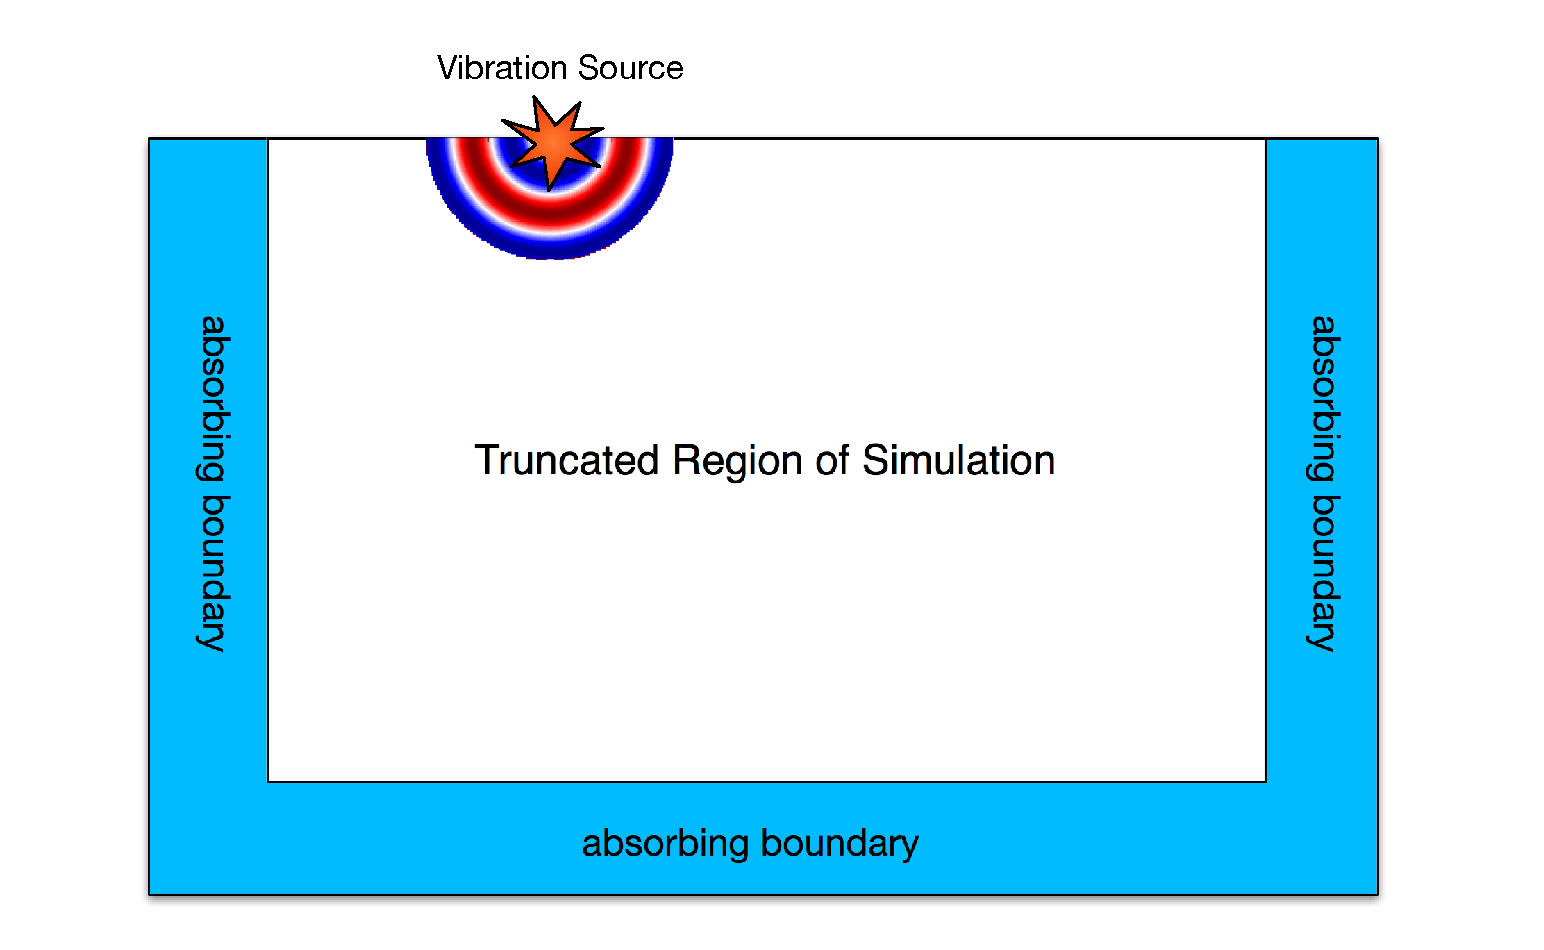
\includegraphics[width=0.6\textwidth]{Fig/ABC}
\caption{Absorbing boundaries of a 2-D simulation region}
\label{fig:ABC}
\end{figure}

Numerically, a simple but efficient method for the ABC is called sponge ABC \cite{Cerjan:1985aa}. As its name suggests, the reflections are exponentially attenuated in the extended artificial boundary area by multiplying a factor $d(u) < 1$.
\begin{equation}
d(u) = e^{-\alpha^2\text{dist}(u)^2}, \mbox{  where  } u=x, z
\end{equation}
where $\text{dist}(u)$ is the distance from $u$ to the original boundary in the $u$ direction. 

The source file which implements the acoustic wave propagation with sponge ABC is \path{src/fwdTimeSpongeFor2dAw.m}. Throughout of the source files in the S3I,  we follow the following naming rules: \path{fwd} means forward (\path{rvs} means reverse); \path{Time} means the equation is solved in the time domain (\path{freq} means in frequency domain); \path{For2d} means 2-D (\path{For3d} means 3-D); and \path{Aw} is short for acoustic wave (\path{Ew} is for elastic wave).  Although the waves are considerably attenuated by ABC, the reflection still can not be completely eliminated. This is the motivation in the S3I we utilize the method called Perfectly Matched Layer as well.


\subsubsection{Perfectly Matched Layer (PML)}
The Perfectly Matched Layer (PML) method was originally formulated for use of electromagnetic equations. In seismic simulations the PML is proven to be effective for wave equations (both acoustic and elastic) as well \cite{Komatitsch:2007aa}. It has a zero reflection coefficient for all angles of incidence and all frequencies before discretization. Moreover, a PML interface between a physical medium and the extended artificial boundary completely absorbs incident waves from the physical medium regardless of its incidence angle and frequency. By defining a damping profile $d(u)$ ($u=z, x, y$) function (see \path{src/dampPml.m}) such that $d(u) = 0$ inside the physical medium and $d(u) > 0$ in the PML region, a new complex coordinate $\tilde{u}$ is introduced as
  \begin{equation}
  \label{eq:replace}
  \tilde{u}(u) = u + \frac{1}{j\omega}\int_0^u d(s)\mathrm{d}s.
  \end{equation}
Equivalently,
  \begin{equation}
  \frac{\partial}{\partial \tilde{u}} = \frac{j\omega}{j\omega + d(u)}\frac{\partial}{\partial u} = s_u(j\omega)\frac{\partial}{\partial u}.
  \end{equation} 
  
\begin{figure}[htbp]
\centering
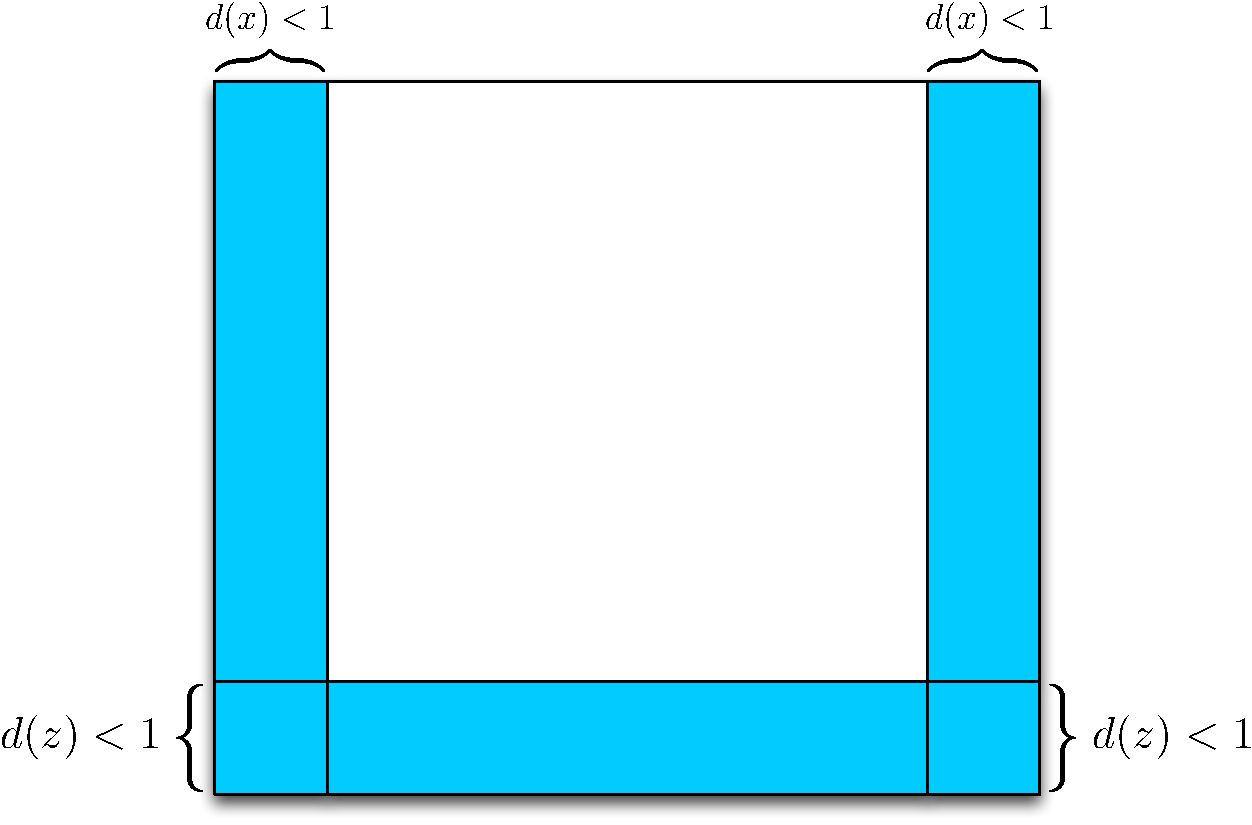
\includegraphics[width=0.7\textwidth]{Fig/SpongeABC.pdf}
\caption{The damping profile $d(u)$}
\end{figure}
In homogeneous media, the acoustic wave equation has a solution
 \begin{equation}
 A \exp(-j (\bk \cdot \bx -\omega t))
 \end{equation}
  where $A$ represents the amplitude and polarization of the plane wave. The $\bk = k_x \hx + k_y \hy +k_z \hz$ denotes the wave vector, which indicates the direction of wave propagation of the plane wave. $\bx = x\hx +y\hy +z \hz$ is the position vector. By substitution  in \eqref{eq:replace}, we can derive another solution of the acoustic equation
\begin{equation}
\begin{aligned}
&A\exp(-j(k_x \tilde{x} + k_y y + k_z z -\omega t))=\\
 &~~~~~~~~~~~~A\exp(-j (\bk\cdot \bx -\omega t))\exp(-kx/\omega \int_0^x d(s)ds).
\end{aligned}
\end{equation}
In the original simulated region the the new solution is equivalent to the old one, since $d_x=0$. Additionally, in the $\hat{\mathbf{n}}= \hx$ direction, the wave amplitude decay with a coefficient $\exp(-kx/\omega \int_0^x d(s)ds)$ that is inversely proportional to the angular frequency $\omega$ of the plane wave. 

In the S3I we implement a non-split method, the Convolutional PML (CPML) \cite{Luebbers:1992aa, Roden:2000aa, Komatitsch:2007aa}, which is more natural for an acoustic (pressure) source function. In time domain,
 \begin{equation}
    \frac{\partial}{\partial \tilde{u}} = s_u(t) * \frac{\partial}{\partial u} = \frac{\partial}{\partial u} - \left(d(u)H(t)e^{-d(u)t}\right) * \frac{\partial}{\partial u}.
  \end{equation}
The convolution can be performed as follows,
  \begin{equation}
  \label{eq:fwdTimeCpml}
  \left\{
  \begin{aligned}
  &\frac{\partial^2 p}{\partial t^2}=v^2(P_z+P_x)\\
  &P_z=\frac{\partial A_z}{\partial z}+\Psi_z\\
  &P_x=\frac{\partial A_x}{\partial x}+\Psi_x\\
  &A_z=\frac{\partial p}{\partial z}+\Phi_z\\
  &A_x=\frac{\partial p}{\partial x}+\Phi_x
  \end{aligned}
  \right.
  \end{equation}
  and  
  \begin{equation}
  \label{eq:fwdTimeCpml_var}
  \left\{
  \begin{aligned}
  &\Psi_z^{(n)}=b_z\Psi_z^{(n-1)}+(b_z-1)\partial_z^{(n-1)}A_z\\
  &\Psi_x^{(n)}=b_x\Psi_x^{(n-1)}+(b_x-1)\partial_x^{(n-1)}A_x\\
  &\Phi_z^{(n)}=b_z\Psi_z^{(n-1)}+(b_z-1)\partial_z^{(n-1)}p\\
  &\Phi_x^{(n)}=b_x\Phi_x^{(n-1)}+(b_x-1)\partial_x^{(n-1)}p\\
  &b_z = e^{-d(z)\Delta t}\\
  &b_x = e^{-d(x)\Delta t}
  \end{aligned}
  \right.
  \end{equation}

The implementations of acoustic wave propagation with CPML are \path{src/fwdTimeCpmlFor2dAw.m} and \path{src/fwdTimeCpmlFor3dAw.m}. For higher efficiency of the simulation, the \path{fwdTimeCpmlFor2dAw.m}, which is used frequently in the seismic imaging algorithms, is also implemented with C MEX-files. 


\subsection{Parallel Computing Using OpenMPI}
Parallel computing based on the distributed memory model is supported in the S3I. One can run our code on a computer cluster across multiple computing nodes. As is shown in Figure \ref{fig:distrMemModel}, these computing nodes can be regarded as separate computers connected by a fast network. Each node has its own independent processor(s) and memory, takes charge of its own calculations and communicates with its direct neighboring nodes.
\begin{figure}[htbp]
\centering
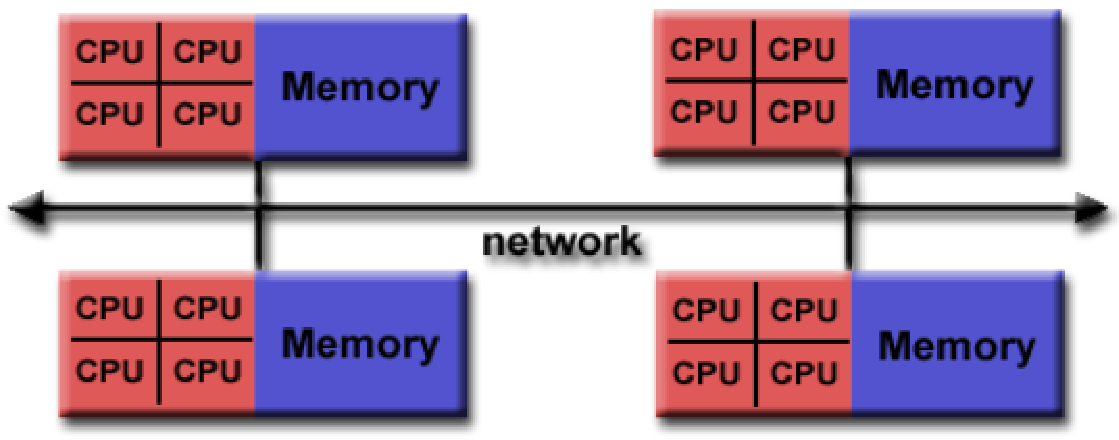
\includegraphics[width=0.7\textwidth]{Fig/MPI_MultipleCPU.pdf}
\caption{Distributed memory model of a computer cluster}
\label{fig:distrMemModel}
\end{figure}

Parallel computing for distributed memory model requires passing messages among different nodes. The standard protocol to achieve this requirement is Message Passing Interface (MPI) of which there are various implementations for different programming languages. The S3I uses OpenMPI\cite{Gabriel:2004aa} that has been widely accepted by many TOP500 supercomputers to implement distributed-memory parallelism and achieves high efficiency.

In MPI parallel computing, the same program runs on all computing nodes independently after it is correctly compiled by \texttt{mpicc}. Each node is assigned a unique identifying number (called "rank"), and the program source code can include logic so that different code paths are followed on different nodes. Since MPI operates in a distributed fashion, any message transfer between nodes must be done explicitly via routine calls provided by OpenMPI, such as \texttt{MPI\_Send}, \texttt{MPI\_Recv}, \texttt{MPI\_Scatter}, \texttt{MPI\_Gather}, etc.
\begin{figure}[htbp]
\centering
  \subfloat[2-D data division]
  {
    \begin{minipage}{0.45\linewidth}
      \begin{tikzpicture}[scale=0.85, every node/.style={scale=0.85}]
      \draw[thick,->] (-0.25, -0.25) -- (1, -0.25) node[anchor=north west] {x};
      \draw[thick,->] (-0.25, -0.25) -- (-0.25, 1) node[anchor=south east] {z};
      \draw[dashed] (0.5, 4) -- (0, 4) -- (0, 0) -- (0.5, 0);
      \draw (0.5, 0) rectangle (4.5, 4);
      \draw[dashed] (4.5, 4) -- (5, 4) -- (5, 0) -- (4.5, 0);
      \draw[red, dashed] (1, 4) -- (1, 0);
      \draw[red, dashed] (2, 4) -- (2, 0);
      \draw[red, dashed] (3, 4) -- (3, 0);
      \draw[red, dashed] (4, 4) -- (4, 0);
      \draw[red, thick,<-] (2.5, -0.5) -- (2.5, -1) node[anchor=north] {Partition};
      \end{tikzpicture}
    \end{minipage}
    \label{fig:division2d}
  }
  \hspace{1em}
  \subfloat[3-D data division]
  {
    \begin{minipage}{0.45\linewidth}
      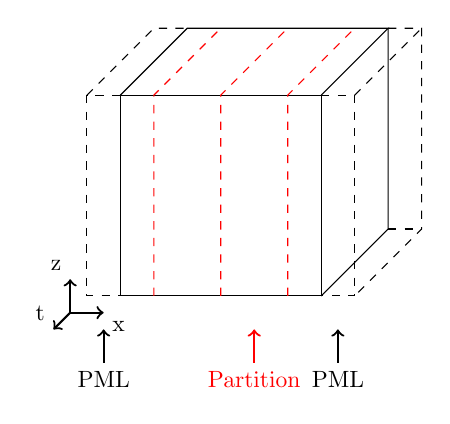
\begin{tikzpicture}[scale=0.85, every node/.style={scale=0.85}]
      \draw[thick,->] (-0.25, -0.25) -- (0.25, -0.25) node[anchor=north west] {x};
      \draw[thick,->] (-0.25, -0.25) -- (-0.25, 0.25) node[anchor=south east] {z};
      \draw[thick,->] (-0.25, -0.25) -- (-0.5, -0.5) node[anchor=south east] {t};
      \draw[dashed] (0.5, 3) -- (0, 3) -- (0, 0) -- (0.5, 0);
      \draw[dashed] (0, 3) -- (1, 4) -- (1.5, 4);
      \draw[thick,<-] (0.25, -0.5) -- (0.25, -1) node[anchor=north] {PML};
      \draw (0.5, 0) rectangle (3.5, 3);
      \draw (0.5, 3) -- (1.5, 4) -- (4.5, 4) -- (3.5, 3);
      \draw (4.5, 4) -- (4.5, 1) -- (3.5, 0);
      \draw[dashed] (3.5, 3) -- (4, 3) -- (4, 0) -- (3.5, 0);
      \draw[dashed] (4.5, 4) -- (5, 4) -- (5, 1) -- (4, 0);
      \draw[dashed] (4, 3) -- (5, 4);
      \draw[dashed] (4.5, 1) -- (5, 1);
      \draw[thick,<-] (3.75, -0.5) -- (3.75, -1) node[anchor=north] {PML};
      \draw[red, dashed] (1, 0) -- (1, 3) -- (2, 4);
      \draw[red, dashed] (2, 0) -- (2, 3) -- (3, 4);
      \draw[red, dashed] (3, 0) -- (3, 3) -- (4, 4);
      \draw[red, thick,<-] (2.5, -0.5) -- (2.5, -1) node[anchor=north] {Partition};
      \end{tikzpicture}
    \end{minipage}
    \label{fig:division3d}
  }
\caption{Workload Division}
\label{fig:division}
\end{figure}

In the S3I, the acoustic wave propagation process can be simulated in such a parallel manner. Suppose there are $P$ nodes, each node $p$ ($p=0, 1, \dots, P-1$) takes over a local partition from two-dimensional velocity model $\left\{v_{i,j}\right\}$ and three-dimensional input source term $\left\{f_{i,j}^{(n)}\right\}$ to perform the simulation locally. Assuming that all nodes have similar computational capacity, these local partitions can be almost evenly divided along the x-axis as follows, 
\begin{equation}
  \label{eq:mpiWorkDivision}
  n_{x_p} = \left\{
  \begin{aligned}
    \left\lfloor \frac{n_x}{P} \right\rfloor + 1, \quad &\text{if } p < \bmod(n, P) \\
    \left\lfloor \frac{n_x}{P} \right\rfloor, \quad &\text{else}
  \end{aligned}
  \right.
\end{equation}
where $n_{x_p}$ is x-axis length of the local partition assigned to node $p$ and $n_x$ is the total x-axis length of velocity model and input source term including the thickness of PML on both left and right sides. Such a workload division process can be demonstrated in Figure \ref{fig:division} where local partitions are separated by red dash lines. From the 1st-order finite difference approximation of wave equation in \eqref{eq:stagGrid}, we can observe that the calculation of any grid value on the next time step $p_{i,j}^{(n+1)}$ only depends on the values of its four direct neighboring grids on the current time step $p_{i-1,j}^{(n)}$, $p_{i+1,j}^{(n)}$, $p_{i,j-1}^{(n)}$, $p_{i,j+1}^{(n)}$, and its value on the current and previous time step $p_{i,j}^{(n)}$, $p_{i,j}^{(n-1)}$, respectively. In our practical simulations, the forward P-wave propagation process is simulated by \eqref{eq:fwdTimeCpml} and \eqref{eq:fwdTimeCpml_var} where $\partial_z$ and $\partial_x$ is approximated by a weighted sum of finite differences described in \eqref{eq:weight}. Hereby values of more neighboring grids on the current time step are involved. While calculating the grid values along the boundary of each partition, their neighboring grid values involved in the calculation only exist in the previous or next partition which is stored in another node. Therefore, in order to avoid calculation error, these grid values must be transferred via MPI before they are needed. The final global result will be gathered after all nodes finish calculations of their own partitions.

Parallel forward and backward acoustic wave propagation is implemented in \path{src/fd_cmex/fwdTimeCpmlFor2dAw_openmpi_mex.c} and \path{src/fd_cmex/rvsTimeCpmlFor2dAw_openmpi_mex.c}, respectively. In order to evaluate the performance, a MATLAB wrapper interface \path{mainRtmTimeCpmlFor2dAwOpenMPI.m} sets up simulation parameters. One can call 
\begin{lstlisting}[basicstyle=\ttfamily,keywordstyle=\color{blue}]
mpirun -n <NP> matlab -nodisplay -r
"mainRtmTimeCpmlFor2dAwOpenMPI"
\end{lstlisting}
in the console to run the parallel forward acoustic wave propagation, where \texttt{<NP>} refers to the number of processors to use.


\subsection{Numerical Artifacts and Instabilities}
In seismic simulations, there are a number of parameters whose values need to be specified, such as the grid spacing, source function frequency, sampling rate, etc. For the stability and accuracy of the numerical scheme, some premises should be honored when we adjust these parameters. Particularly, when Nyquist sampling criteria for the finite difference wave field simulation has not been satisfied in space or time domain, some numerical artifacts and instabilities will occur. In summary, when the spatial sampling rate is too low,  the solution suffers numerical grid dispersion; when the temporal sampling rate is too low, the Courant instability happens.

To avoid the occurrence of harmful grid dispersion the following criteria for the spatial grid spacing $\Delta u$ has to be satisfied
\begin{equation}
  \Delta u \leq \frac{\lambda_{\min}}{n} = \frac{V_{\min}}{nf_{\max}}
\end{equation}
where $n$ is the number of sampling points per wavelength, $\lambda_{\min}$ and $V_{\min}$ are the minimal wave length and velocity, and $f_{\max}$ is the maximal frequency. Video clips of acoustic wave propagation with and without numerical grid dispersion can be found at: \url{https://www.youtube.com/watch?v=scBvd3FQ73U} and \url{https://www.youtube.com/watch?v=Q17tieZuhJQ}

To be Courant stable, the time step $\Delta t$ must be less than the time for the wave to travel between two adjacent sampling points with grid spacing $\Delta u$. In 2-D scenarios,
\begin{equation}
\frac{\sqrt{2}V_{\textbf{max}}\Delta t}{\min\{\Delta z, \Delta x\}}\le \epsilon \le 1.
\end{equation}
Examples of acoustic wave propagation which are Courant stable and Courant instable can be found at \url{https://www.youtube.com/watch?v=Gl1pNm3jF8g} and \url{https://www.youtube.com/watch?v=wMAuhW7gzdM}. In the Courant instable case, noting the color bar, the solution actually blows up over time.

An approach to alleviate the numerical dispersion is flux-corrected transport (FCT) introduced by \cite{Fei:1995aa}, which is implemented for both acoustic and elastic waves in the S3I (see \path{src/fctForAw.m} and \path{src/fctForEw.m}). In the default simulations of acoustic and elastic waves the FCT correction is turned off, since it can slow down the simulation significantly. If possible, we strongly suggest to modify the sampling rate and $\Delta u$ to avoid the grid dispersion rather than employing FCT.  


\subsection{2D Acoustic Wave Equation in Frequency Domain}
In signal processing, a signal transformed into frequency domain may unveil hidden information in time domain and brings new processing techniques. The acoustic wave equation given in \eqref{eq:aw} which is time dependent can be transformed and solved in frequency domain as well. Taking Fourier transform of \eqref{eq:aw} with respect to $t$ on both sides, we obtain
  \begin{equation}
  \frac{\omega^2}{c^2(z, x)}P_{\omega}(z, x) + \nabla^2 P_{\omega}(z, x) =- F_{\omega}(z, x).
  \end{equation}
 The spatially discretization of the simulated region is the same grid as we set for the FDM in time domain. Let $P_{i,j}^{(\omega)} := P_{\omega}(i\Delta z, j\Delta x)$, $F_{i,j}^{(\omega)} := 
  F_{\omega}(i\Delta z, j\Delta x)$, $c_{i,j} := c(i\Delta z, j\Delta x)$  with 1st-order finite difference approximation of the Laplace operator. We obtain the following discrete equation for a specific frequency $\omega$
  \begin{equation}
  \begin{aligned}
  \frac{\omega^2}{c_{i,j}^2} P_{i,j}^{(\omega)} &+\left[ \frac{P_{i-1,j}^{(\omega)} - 2P_{i,j}^{(\omega)} + P_{i+1,j}^{(\omega)}}{\Delta z^2} \right] \\&+\left[ \frac{P_{i,j-1}^{(\omega)} - 2P_{i,j}^{(\omega)} + P_{i,j+1}^{(\omega)}}{\Delta x^2} \right] =- F_{i,j}^{(\omega)}.
  \end{aligned}
  \end{equation}
  
There are some advantages of Finite Difference in Frequency Domain (FDFD) over Finite Difference in Time Domain (FDTD) that we will discuss shortly. The Fourier transform convert the second-order derivative with respect to $t$ in the wave equation into a product. So the wave field at a certain frequency $\omega$ is determined by a system of linear equations 
\begin{equation}\label{eq:awFreq}
\bA^{(\omega)}\bp^{(\omega)} = \bff^{(\omega)},
\end{equation}
where $\bff^{(\omega)}$ and $\bp^{(\omega)}$ are the vectorized source term $F_{i,j}$ and pressure field $P_{i,j}$.
 \begin{figure}[htbp]
\centering
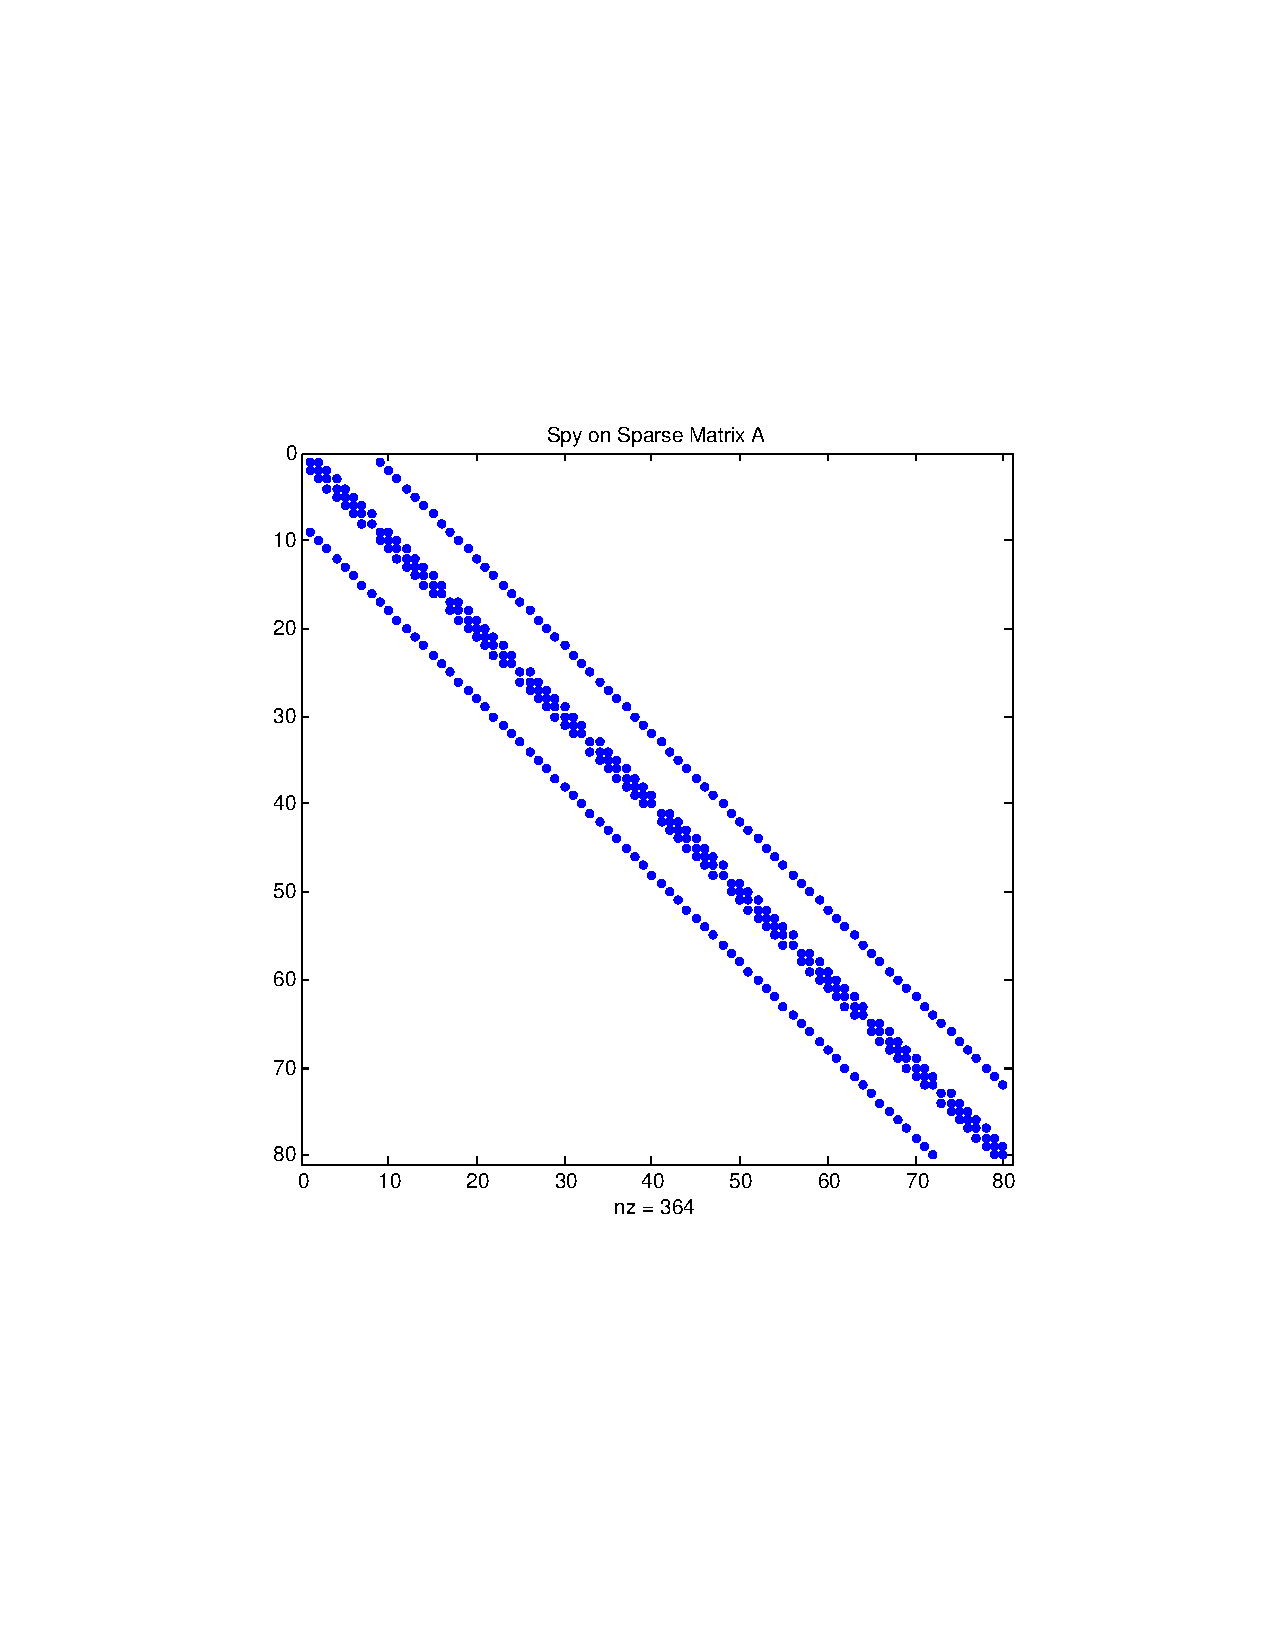
\includegraphics[width=0.5\textwidth]{Fig/FDFDMatrixA.pdf}
\caption{sparse FDFD matrix $\bA$ for a specific frequency $\omega$. Blue dots denote the nonzero elements.}
\label{fig:SparseA}
\end{figure}

The matrix $\bA$ is highly sparse (see Figure \ref{fig:SparseA}), because $P_{i,j}$ is only dependent on its adjacent grid points and such that each row of $\bA$ contains at most five nonzero entries. MATLAB has been optimized to invert the sparse matrix. Other than the tool come along with MATLAB, when the size of $\bA$ is huge, we recommend a well developed package with a MATLAB interface called MUMPS (MUltifrontal Massively Parallel sparse direct Solver) to solve the sparse matrix inversion problem. The concerns on data storage and process is another factor which made FDFD excels FDTD for our application. Instead of processing the whole data set in time domain, we can solve the wave equation only in the important part of spectrum using FDFD, which considerably reduces the size of the data and makes large-scale problems (e.g., full waveform inversion) feasible. Since the wave equations are independent over frequencies, FDFD can be easily parallelized across frequencies to achieve a better processing speed.


An interesting example is the Green's function, which is the solution of wave equation with an impulse source term. Numerically, the Green's function cannot be solved accurately using FDTD, because the impulse function has components in arbitrarily high frequency. The impulse source function brings serve grid dispersion to the numerical solution. However this is not an issue at all for FDFD. The Green's Function $G_{\omega}$ in frequency domain, which solves  
  \begin{equation}
  \frac{\omega^2}{c^2(z, x)}G(z, x;\omega) + \nabla^2 G(z, x;\omega) = \delta_{\omega}(z-z_0, x-x_0)
  \end{equation}
  is a the solution of \eqref{eq:awFreq} with the source term $\bff$ contains all one's.
  
\begin{figure}[htbp]
\centering
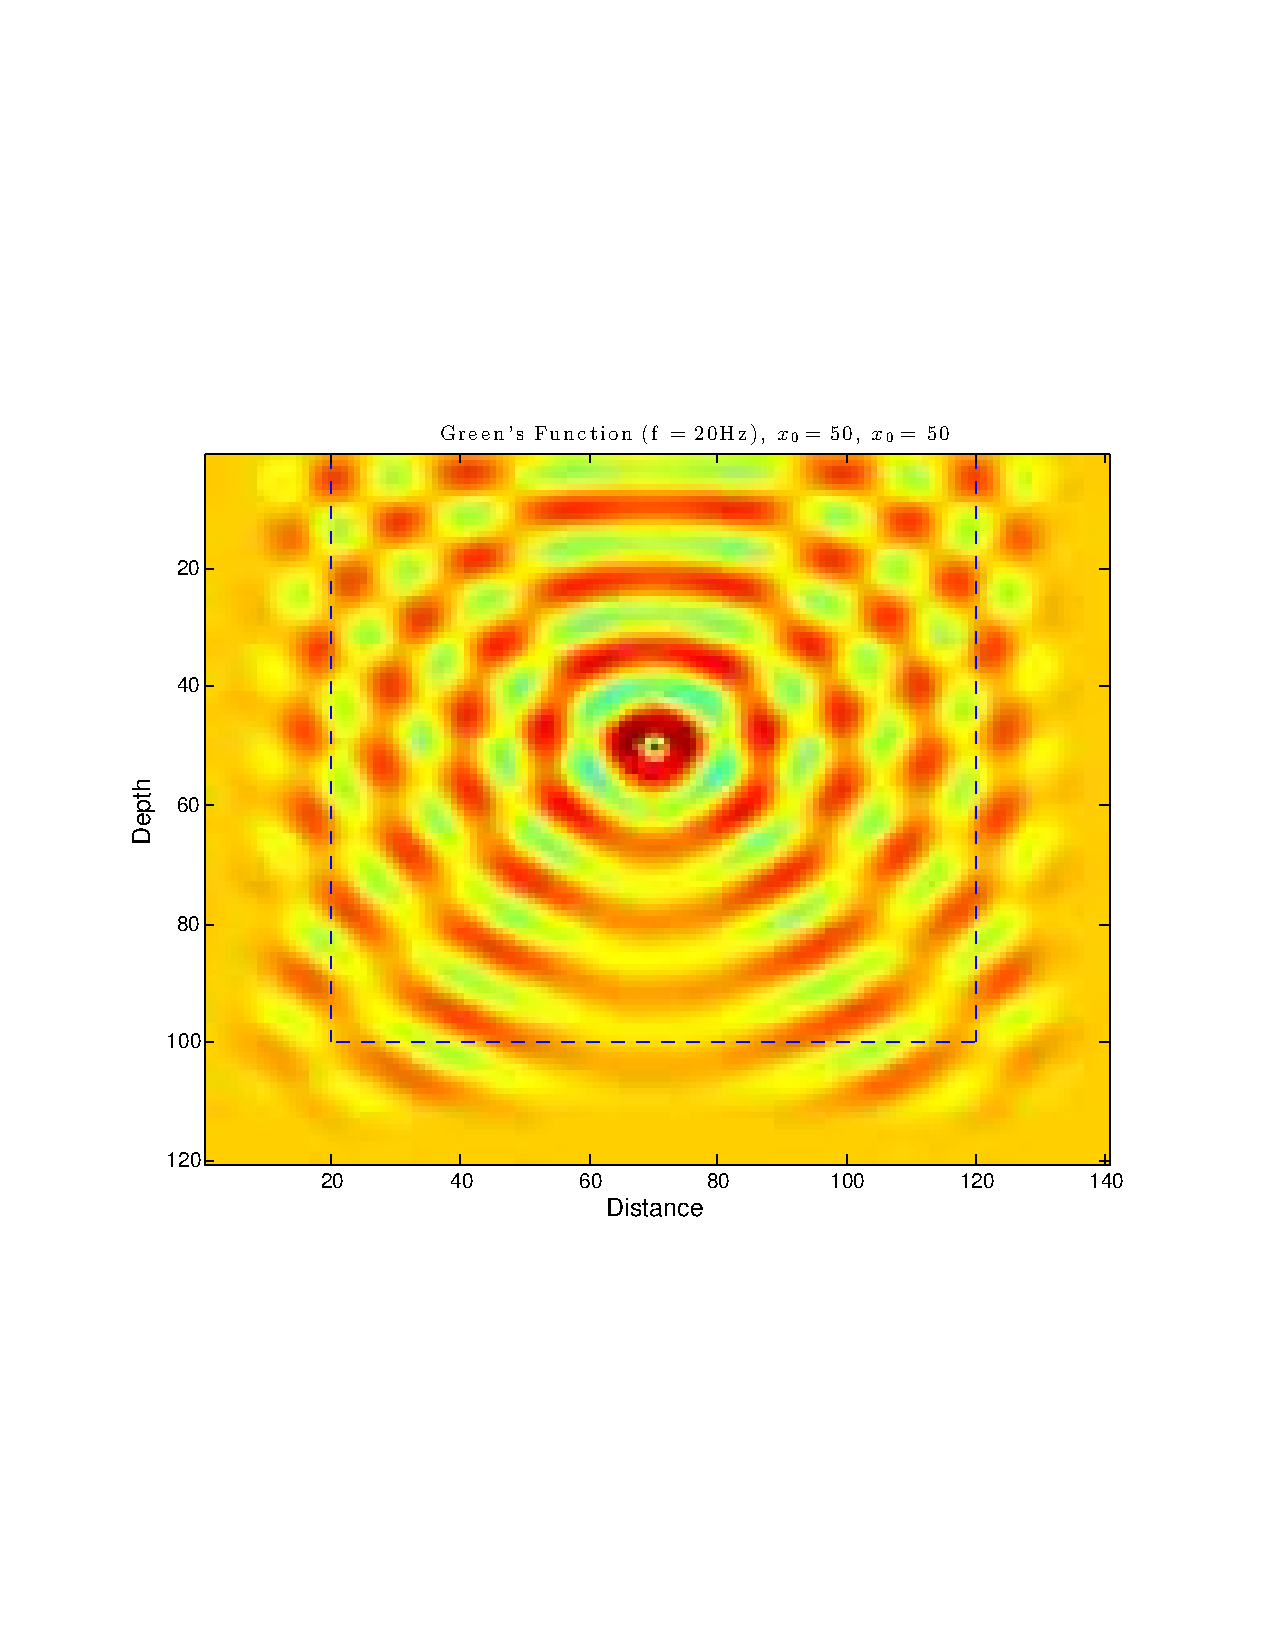
\includegraphics[width=0.5\textwidth]{Fig/GreensFunction.pdf}
\caption{Real part of the Green's function at frequency 20 Hz for a region with PML} 
\end{figure}



\section{Numerical Solution for Elastic Wave Equation}
In the real media, the seismic waves are in the form of elastic waves which are composed of both P-wave and S-wave. The particle velocity field satisfies 
\begin{equation}
    \left\{
    \begin{aligned}
    %v_z=\frac{\partial s_z}{\partial t}, \quad &v_x=\frac{\partial s_x}{\partial t}\\
    v_z=v_{zp}+v_{zs}, \quad &v_x=v_{xp}+v_{xs}\\
    \frac{\partial v_{zp}}{\partial t}=\alpha^2 \frac{\partial A}{\partial z}, \quad &\frac{\partial v_{xp}}{\partial t}=\alpha^2 \frac{\partial A}{\partial x}\\
    \frac{\partial v_{zs}}{\partial t}=-\beta^2 \frac{\partial B}{\partial x}, \quad &\frac{\partial v_{xs}}{\partial t}=\beta^2 \frac{\partial B}{\partial z}\\
    A=\frac{\partial s_z}{\partial z}+\frac{\partial s_x}{\partial x}, \quad &B=\frac{\partial s_x}{\partial z}-\frac{\partial s_z}{\partial x}
    %\frac{\partial A}{\partial t}=\frac{\partial v_z}{\partial z}+\frac{\partial v_x}{\partial x}, \quad& \frac{\partial B}{\partial t}=\frac{\partial v_x}{\partial z}-\frac{\partial v_z}{\partial x} 
    \end{aligned}
    \right.
    \end{equation}
  where $(v_z, v_x)$ is the particle velocity field, $v_{up}$ is P-wave field in $u$-direction $(u=x, z)$, $v_{us}$ is the S-wave fields in $u$-direction $(u=x, z)$, and $(s_z, s_x)$ is particle displacement vector. We can see that in this form the P-wave and S-wave fields are separated in the solution \cite{Chen:2014aa}. Thus a split PML (SPML) for the FDFD is adopted in S3I (see \path{src/fwdTimeSpmlFor2dEw.m}).
    
\begin{figure}[htbp]
\centering
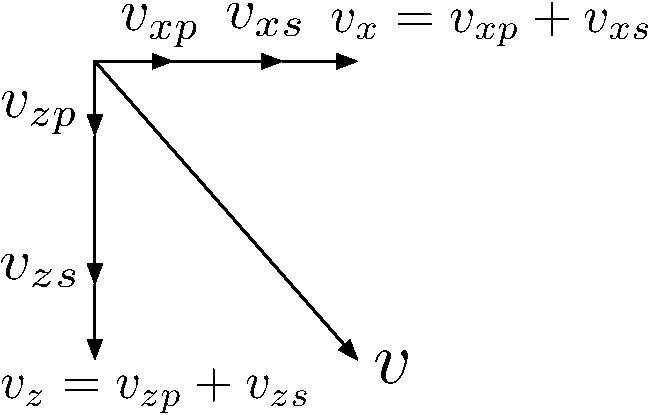
\includegraphics[width=0.5\textwidth]{Fig/EWCoordinates.pdf}
\caption{Velocity separation}
\end{figure}



\section{Migration}
The goal of seismic imaging is to recover the subsurface structures with the recorded seismic data. This imaging process is typically computationally intense. Migration is one of the most important approaches. In the S3I we implemented a few common migration algorithms, such as Kirchhoff's migration, Reverse Time Migration (RTM), and Least square RTM (LSRTM). All methods we implemented in the S3I are prestack.  


\subsection{Kirchhoff's Migration}
Let $\bx_r$ be the location of the receiver and $\bx_s$ be the location of the source. Then $\bm=(\bx_r+\bx_s)/2$ is the midpoint, and $\bh=(\bx_r-\bx_s)/2$ is the half offset. The involved derivation of Kirchhoff's migration (see \cite{Schneider:1978aa} for details) is omitted here. Only the simple imaging formula is given as below
\begin{equation}
\label{eq:kirchhoffImaging}
I(\xi)=\int_{\Omega_\xi} W(\xi,\bm,\bh)dt(t=t_d(\xi,
\bm,\bh),\bm,\bh)d\bm d\bh,
\end{equation}
where limited region $\Omega_\xi$ is centered around the location $\xi$ in the $m$ plane, called the migration aperture. $t_d=t_s[\bx,\bs,v(z,x,y)]+t_r[\bx,\bg,v(z,x,y)]$, where $t_s$ is the travel time from the reflector $\xi$ to $\bx_s$ and $t_r$ is the travel time from $\xi$ to $\bx_r$, see Figure \ref{fig:ref}. For reflector $\xi = (z_\xi, x_\xi, y_\xi)$ in 3-D and $\xi = (z_\xi, x_\xi)$ in 2D case.

\begin{figure}[htbp]
\centering
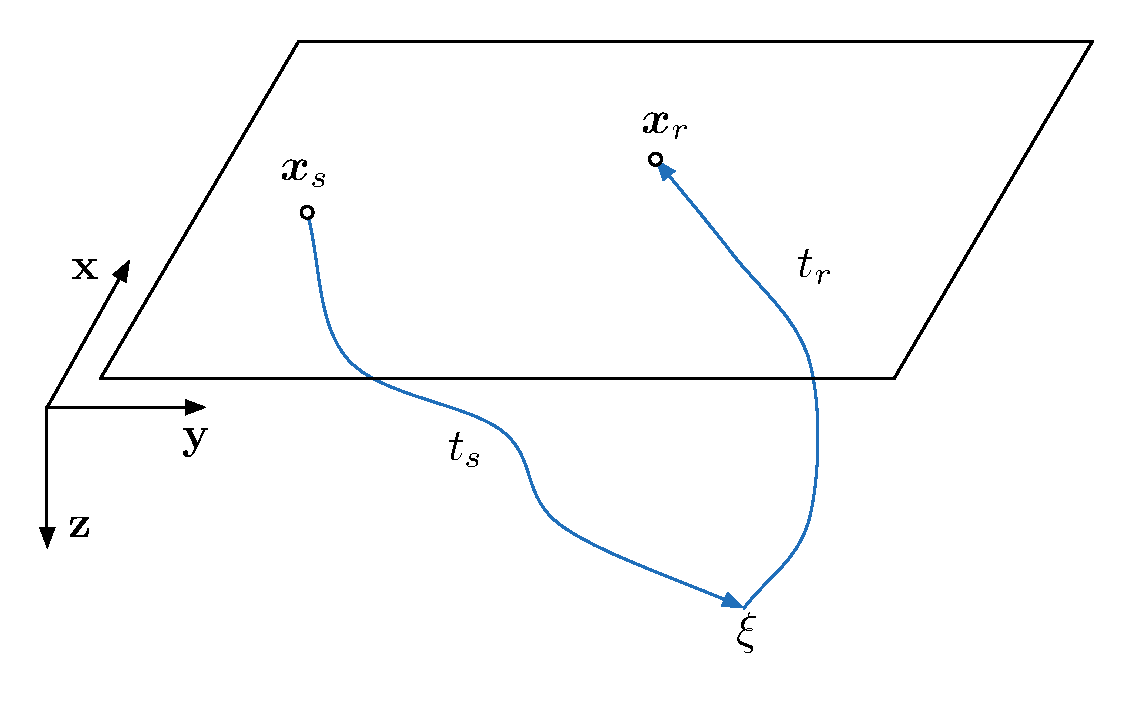
\includegraphics[width=0.5\textwidth]{Fig/tstr}
\caption{Reflector, and travel time}
\label{fig:ref}
\end{figure}
  
An example of Kirchhoff's migration (see Figure \ref{fig:kirc}) for the fault model or Marmousi model (available in the \path{modelData} folder) can be found in \path{mainKircCpmlFor2dAw.m}, which is inherited from an existing package \cite{Kozola:2011aa}. The most important part of Kirchhoff's migration is the computation of travel times $t_s$ and $t_r$. These can be done either with \path{src/ray2d.m} from \cite{Kozola:2011aa} or \path{src/eikonal2d.m} which solves the 2-D Eikonal equation using a fast sweeping method \cite{Zhao:2004aa}.

\begin{figure}
\centering
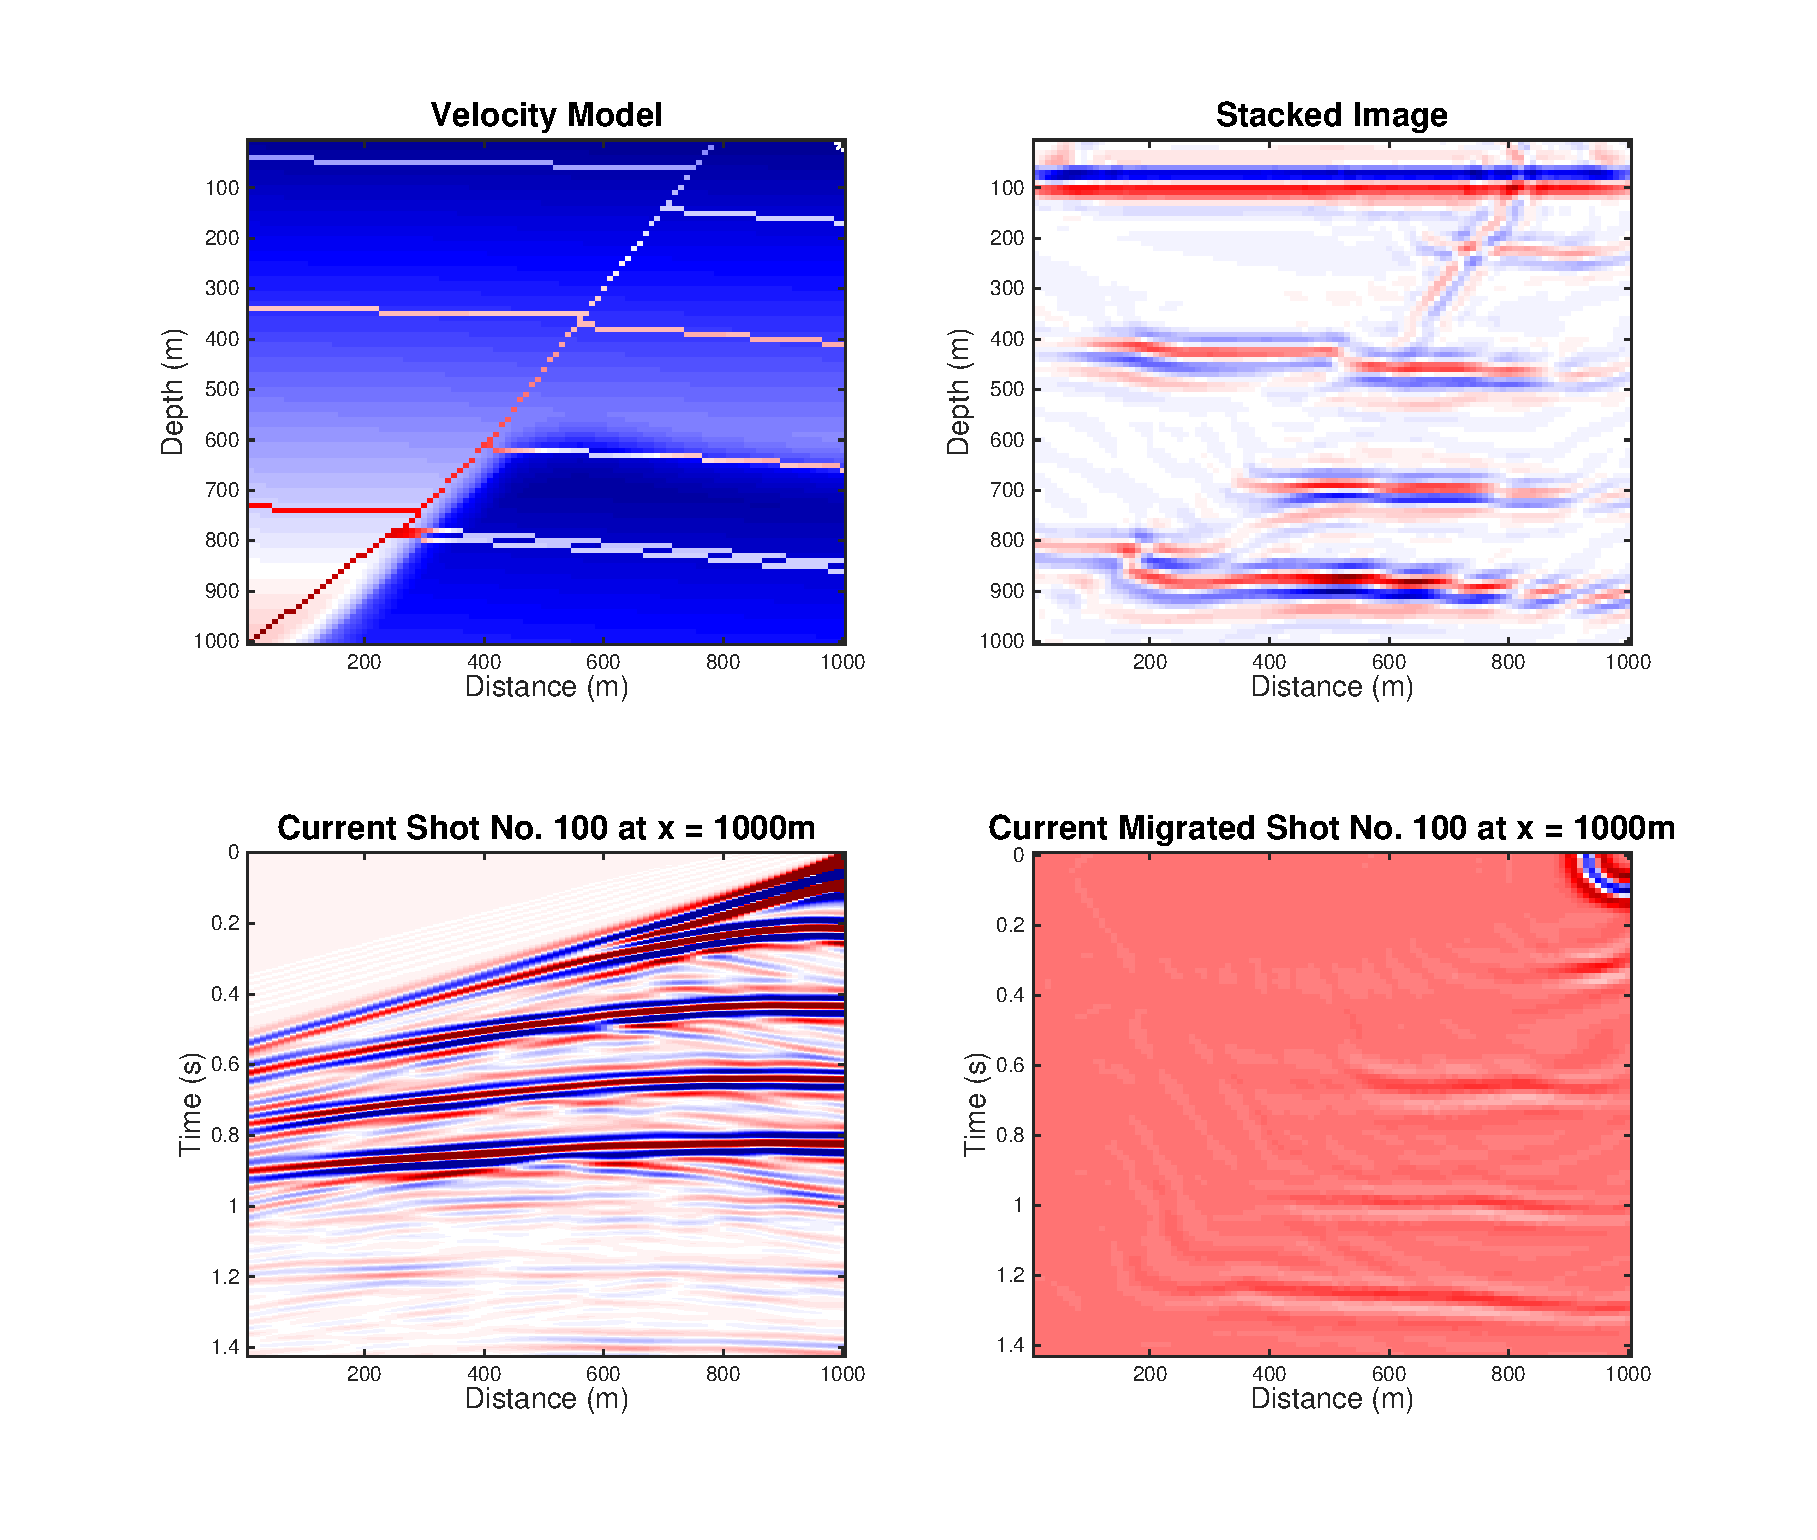
\includegraphics[width=0.9\textwidth]{Fig/kirc.eps}
\caption{Kirkchhoff's migration result of the faults model}
\label{fig:kirc}
\end{figure}

The Eikonal equation is of the form
\begin{equation}
|\nabla T(\bx)| v(\bx)= 1, ~~\bx\in \real^2
\end{equation}
subject to $T(\bx) = 0$ for a boundary $\Gamma$. In the S3I we consider the source point to be a single grid point $\bx_s$. When we solve the Eikonal equation in a truncated region, $T(\bx)$ gives the time of first arrival in this region. 


\subsection{Reverse Time Migration (RTM)}
The Reverse Time Migration (RTM) is a two-way wave-equation migration for accurate imaging in and below areas with complex subsurface structure. In the literature RTM has a relatively old origin, however it has not been used routinely until recently because of its computational intensity. In RTM a forward wave propagation and a reverse wave propagation need to be simulated, which requires a lot of computation power. However, RTM has a number of advantages over conventional depth migration methods, e.g. handing evanescent energy and no dip limitation \cite{McMechan:1983aa, Baysal:1983aa}. In summary, RTM is implemented in three steps. 
\begin{enumerate}
  \item record forward wave field $p_f(\bx, t; \bx_s)$ through the true velocity model
  \item solve the reverse wave field $p_r(\bx, t)$ by the received surface data through the incident model, which is typically a smoothed version of the true model
  \item combine the above using an imaging condition (chosen from a number existing imaging conditions)
\end{enumerate}
Physically, there is no wave field propagates backward in time. It is only for the purpose of imaging. The second step above is equivalent to reverse the recorded traces in time then input those traces as source functions and solve a forward wave field. 

For instance, an imaging condition using cross-correlation is 
\begin{equation}
\label{eq:rtmImaging}
I(\bx) = \sum_{\bx_s} \frac{\int_0^T p_f(\bx, t; \bx_s)p_r(\bx, t)\mathrm{d}t}{\int_0^T |p_f(\bx, t; \bx_s)|^2\mathrm{d}t + \epsilon^2}.
\end{equation}
Worth noting that using the imaging conditions \eqref{eq:kirchhoffImaging}, \eqref{eq:rtmImaging}, and many other imaging conditions, the values $I(\bx)$ are not necessarily to be meaningful in the model domain. The image $I(\bx)$ only depicts the locations of the reflectors. Based on a migrated image, we may only qualitatively claim that the stronger model perturbation gives greater values in $I(\bx)$. 

\begin{figure}[htbp]
\centering
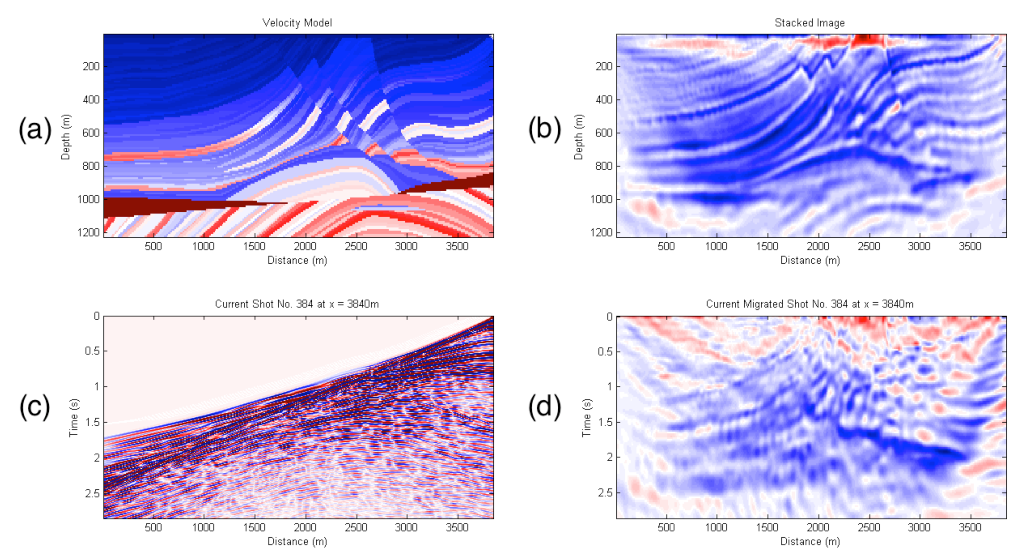
\includegraphics[width=1\textwidth]{Fig/MarmousiRTM.pdf}
\caption{RTM results. (a) Marmousi model, (b) accumulated RTM result; (c) a sample shot record; (d) migrated result of the sample shot. The parameters settings are 15 Hz (center frequency) Ricker wavelet, 384 sensors, 384 shots, grid size $122 \times 384$, $\Delta z = \Delta x = 24$ m.}
\label{fig:RTM}
\end{figure}

The RTM result of Marmousi model is illustrated with Figure \ref{fig:RTM}. Moreover, the aggregating process across source shots for a fault model can be viewed in this video clip
\url{https://www.youtube.com/watch?v=lL-UpW-5xms&feature=youtu.be}. The implementation of RTM is fulfilled using several methods in \path{mainRtmTimeCpmlFor2dAw.m}, \path{mainRtmTimeCpmlFor2dAwOpenMPI.m}, and \path{mainRtmTimeSpongeFor2dAw.m}.



\section{Least Square Reverse Time Migration (LS-RTM)}
Generally speaking, RTM is a reliable method of imaging complex structures. However, there are still some distortions caused by RTM crosstalk artifacts. Mathematically, the migration operator is just the adjoint of the forward modeling operator, it does not minimize the mismatch of the observed and simulated traces. Least Square RTM (LSRTM) introduced by \cite{Nemeth:1999aa} derives an imaging condition by formulating migration as an inverse problem based on a least-squares misfit function. The implementation of LSRTM can either be in time domain or frequency domain\cite{Ren:2013aa}.

Denote by $m(\bx)=1/v^2(\bx)$ the model which is the square slowness at point $\bx$. We consider the decomposition of model $m$ into a smooth model (initial guess) and a perturbation:
\begin{equation}
m(\bx)=m_0(\bx)+\delta m(\bx),
\end{equation} 
where $m_0$ is the smooth model and perturbation $\delta m(\bx) \ll m_0(\bx)$. Accordingly, we split the wave field $p(\bx,t)$ into 
\begin{equation}
p=p_0+\delta p,
\end{equation}
where $p_0$ solves the wave equation in the incident model $m_0(\bx)$. In light of the advantages we have mentioned above, we formulate the problem in frequency domain. For the LSRTM in time domain, one can use the iterative method proposed in \cite{Dong:2012aa}. Similarly, $P(\bx;\bx_s, \omega)$, the waveform generated by source at position $\bx_s$, can also be split into two parts: the incident wavefield $P_0$ and $\delta P$. The $P_0(\bx; \bx_s, \omega)$ is determined by the smooth model and source function via the following acoustic wave equation:
\begin{equation}
\cL( m_0) P_0(\bx; \bx_s, \omega)=F_s(\omega),
\end{equation} 
where operator $\cL( m_0)=(-\omega^2 m_0(\bx)-\Delta)$ and the $F_s(\omega)$ is the source function at source location $\bx_s$. Using Born approximation \cite{Tarantola:1988aa}, the scattered filed can be approximated by  
\begin{equation}
\cL( m_0)\delta P(\bx;\bx_s,\omega) =\omega^2 \delta m P_0(\bx;\bx_s,\omega).
\end{equation}
Let $G(\bx; \bx_s, \omega)$ denote the Green's functions from the shot position $\bx_s$ to a point in the model space $\bx$, which is the solution of 
\begin{equation}
\cL(m_0)G(\bx;\bx_s,\omega)=\delta(\bx-\bx_s).
\end{equation}
It is worth noting that the Green's function $G$ only depends on the smooth model $m_0$. In least square migration, with an accurate smooth model, i.e. initial guess, we can calculate the Green's function and save it for the use of every iteration without updating. 
  
Then the incident field $u_0$ at the surface point $\bx$ becomes
\begin{equation}
P_0(\bx; \bx_s,\omega)=F_s(\omega)G(\bx; \bx_s,\omega).
\end{equation}
And the secondary filed as the surface point $\by$ can be written as 
\begin{equation}
\delta P(\by; \bx_s,\omega)=\omega^2 \sum_{\bx}  \delta m(\bx) P_0(\bx;\bx_s,\omega) G(\by;\bx,\omega).
\end{equation}
For $\by=\bx_r$, we obtain the Born approximation of the synthetic field at the receiver position $\bx_r$. In general, the synthetic data for one frequency $\omega$, a shot positioned at $\bx_s$, and a receiver positioned at $\bx_r$ can be given by a linear operator $L(\bx_s,\bx_r)$ acting on the model $m(\bx)$, as follows:
\begin{align}
\delta P(\bx_r;\bx_s, \omega)&=L(\bx_s,\bx_r)\delta \bm=\omega^2 F_s(\omega)\sum_{\bx}\delta m(\bx)G(\bx;\bx_s,\omega)G(\bx_r;\bx,\omega)\nonumber\\
&=\omega^2 [...,F_s(\omega)G(\bx;\bx_s,\omega)G(\bx_r;\bx,\omega),...]\delta \bm.
\end{align} 
We can write the forward model operator as a $n_s n_r\times K$ ($K$ is the number of grid points) matrix $\bL$
\begin{equation}
\label{eq:operatorL}
\bL(\bx_r;\bx_s,\omega) = \omega^2 [...,L(\bx_s,\bx_r)^*,...]^*.
\end{equation}

The cost function $J$ is the $\ell_2$ norm of the mismatch between the simulated and observed traces
  \begin{equation}
  \begin{aligned}
  %\hspace{-20pt}
  J&(\delta \bm) = \frac{1}{2} \sum\limits_{\omega,\bx_s,\bx_r}  \left| P^{\text{(sim)}}(\bx_r; \bx_s,  \omega) - P^{\text{(obs)}}(\bx_r; \bx_s, \omega) \right|^2 \\
  &= \frac{1}{2} \sum\limits_{\omega,\bx_s,\bx_r} \Big| \omega^2 F_s(\omega) \sum\limits_{\bx}\delta m(\bx)G_{\omega}(\bx; \bx_s)G_{\omega}(\bx_r; \bx) \\&- \delta P^{(obs)}(\bx_r, \bx_s; \omega) \Big|^2\\
  &= \frac{1}{2} \left\| \bL\delta \bm - \delta\bP^{(obs)}\right\|_2^2,
  \end{aligned}
  \end{equation}
where $\delta \bm$ is the model perturbation (roughly saying, the reflectors), $\bL$ is the forward modeling operator. The superscript (sim) means simulated results and (obs) means observed. The optimized model perturbation is 
    \begin{equation}
    \delta \bm^{\text{(opt)}} = \left( \bL^{*}\bL \right)^{-1} \bL^{*} \delta\bP^{(obs)}.
    \end{equation}
Apparently, LSRTM is the simply a preconditioned RTM migration result $\bL^{*}\delta \bP^{(obs)}_{\omega}$. Instead of solving the huge inverse matrix $(\bL^{*}\bL)^{-1}$,  we use the Gauss-Newton method with a diagonal approximation of the Hessian matrix. In the case of large acquisition aperture, wide frequency band, and slow variation of the velocity model, the Hessian matrix is almost diagonal. In a simulation such as Marmousi model, the Hessian matrix is diagonal dominated. 

Concretely, the gradient of the cost function is
\begin{equation}
\bg_k(\delta\bm)=\text{Re}\bigg(\sum_{\omega,\bx_s,\bx_r } \omega^2  \bar{F}_s(\omega) \bar{G}_\omega(\bx;\bx_s)\bar{ G}_\omega(\bx_r;\bx)\Delta d(\bx_r;\bx_s,\omega)\bigg), 
\end{equation}
where $\Delta d(\bx_r;\bx_s,\omega)=\bL\delta \bm - \delta\bP^{(obs)}$. 
As discussed in the preceding sections, the Hessian matrix can be approximated by its diagonal elements.
\begin{equation}
\bH(\bm)= \text{Re}\bigg( \sum_{\omega,\bx_s,\bx_r} \omega^4 |F_s(\omega)|^2 |G_\omega(\bx;\bx_s)|^2 |G_\omega(\bx_r;\bx)|^2 \bigg).
\end{equation} 
Then
\begin{equation}
\delta \bm^{k+1}=\delta \bm^{k} - \bH^{-1} \bg_k(\delta \bm^k),
\end{equation}
where the initial value $\delta \bm^0=\bL^* \delta \bP$ can be obtained using RTM with an imaging condition that maps into the model domain. In the LSRTM, since we do not update the incident model $\bm_0$, the Green's functions and Hessian only need to be computed once and stored for use in the later iteration. Its implementation can be easily modified from the source code for FWI in the next section.



\section{Full Waveform Inversion (FWI) in Frequency Domain}
The migration operator requires an incident model (usually a smoothed version of the true model) as an input. However, in complex media, building an accurate smooth model is challenging. In contrast, the starting model of FWI (see \cite{Virieux:2009aa} as an overview) can be very rough, since in each iteration the updated model will be a new starting point for the following iteration. However, the Green's function should also be updated in order to converge fast. In the frequency domain, the formulation is similar to the LSRTM. The only thing different is we will update the incident model as well as the Green's functions over iterations. Applying the same approach, the cost function $J(\delta \bm)$ can be optimized by conjugate-gradient or quasi-Newton in the model domain or in a sparse domain using Projected Quasi-Newton (PQN) algorithm\cite{Schmidt:2009aa}, see \path{mainAdjointFwiFreqCpmlFor2dAw.m} and \path{mainPQNFwiFreqCpmlFor2dAw.m}.

\begin{algorithm}[H]
\begin{algorithmic}[1]
\WHILE{$m(\bx)$ is not converged}
\STATE Generate Green's functions at each shot and receiver
\STATE Generate scattering wave field $\delta\bP^{(obs)}_{\omega}= \bP_{\omega}^{\text{(obs)}} - \bG_{\omega}(m)\bF_{\omega}$ for all $\omega$
\STATE $\delta \bm^{\text{(opt)}} = \arg\min J(\delta \bm) = \arg\min \frac{1}{2} \left\| \bL(\bm)\delta \bm - \delta\bP^{(obs)}\right\|_2^2$
\STATE $\bm \leftarrow \bm + \delta \bm$
\ENDWHILE
\end{algorithmic}
\caption{Full Waveform Inversion}
\end{algorithm}

For Marmousi model, the result of FWI is illustrated in Figure \ref{fig:FWI}.
\begin{figure}[htbp]
\centering
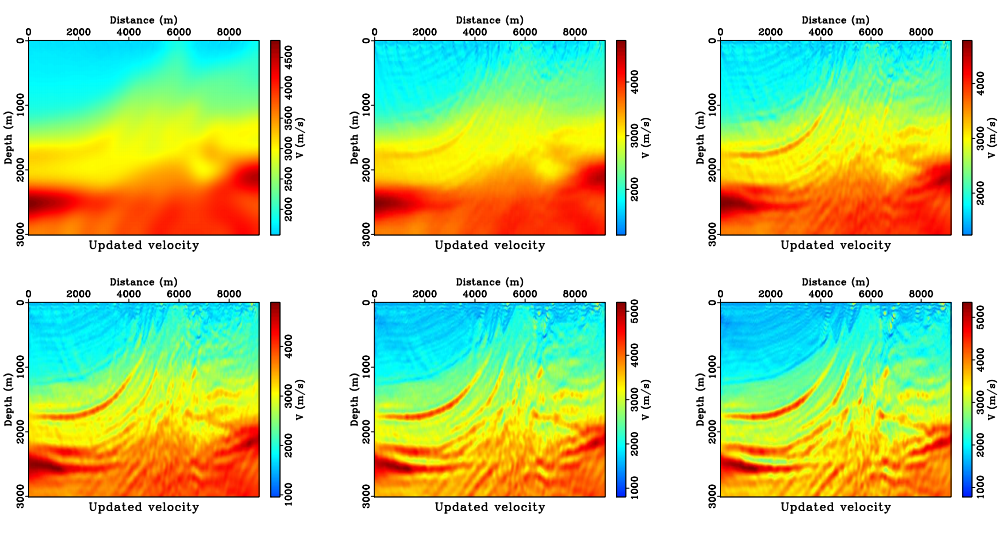
\includegraphics[width=1\textwidth]{Fig/FWI.eps}
\caption{FWI result. (a) Marmousi model (b) starting model (c) FWI results after 15 iterations. The parameters settings are 15 Hz (center frequency) Ricker wavelet, 384 sensors, 384 shots, grid size $122 \times 384$, $\Delta z = \Delta x = 24$ m.}
\label{fig:FWI}
\end{figure}



\section*{Acknowledgement}
\addcontentsline{toc}{section}{Acknowledgement}
Some of the S3I source files are inherited from other open source packages. We are grateful for those contributions. Please read the comments in source files for authorship and contact information. Particularly, we want to thank Stuart Kozola, the author of the package of Large Data in MATLAB: A Seismic Data Processing Case Study\cite{Kozola:2011aa}. His excellent work motivates us to develop the S3I.  



\appendix
\section{Comparison with Other Open Source Packages}
Geophysicists have been working on developing seismic data processing and imaging packages for decades. There are a number of open source packages available online, such as Seismic Unix, SEPLib/SEPLib3d, Madagascar, and CREWES. In part because of this long history, many source code of these packages are written in C and Fortran 77. These code are computationally efficient but with poor readability and extensibility. A comparison in several aspects are illustrated in Figure \ref{fig:comp}. The S3I have the following advantages over the Linux/Unix based packages: 
\begin{enumerate}
  \item Rich functions and toolboxes in MATLAB, e.g. data visualization, data I/O, signal processing, and parallel computing.
  \item Ease of coding and debugging for further development.
  \item Cross-platform: Windows/Linux/Unix.
  \item Easy to use: GUI, simple MATLAB script manipulations, no shell scripting.
  \item Available code reuse: data formatting, spare transforms, advanced optimization algorithms.
\end{enumerate}
Compared with CREWES, which is also based on MATLAB and contains many functions, S3I targets on more specific goals. As its name would suggest, the S3I contains more organized and optimized source code to implement large scale parallel computing and provides a tutorial of the numerical methods in the user guide. It is well known the computing efficiency of MATLAB is not as good as C and Fortran, especially when the code contains a large number of for-loops. Thus, some slow but frequently called functions in S3I are implemented with C MEX-files which significantly speed up the simulation.  

\begin{figure}
\centering
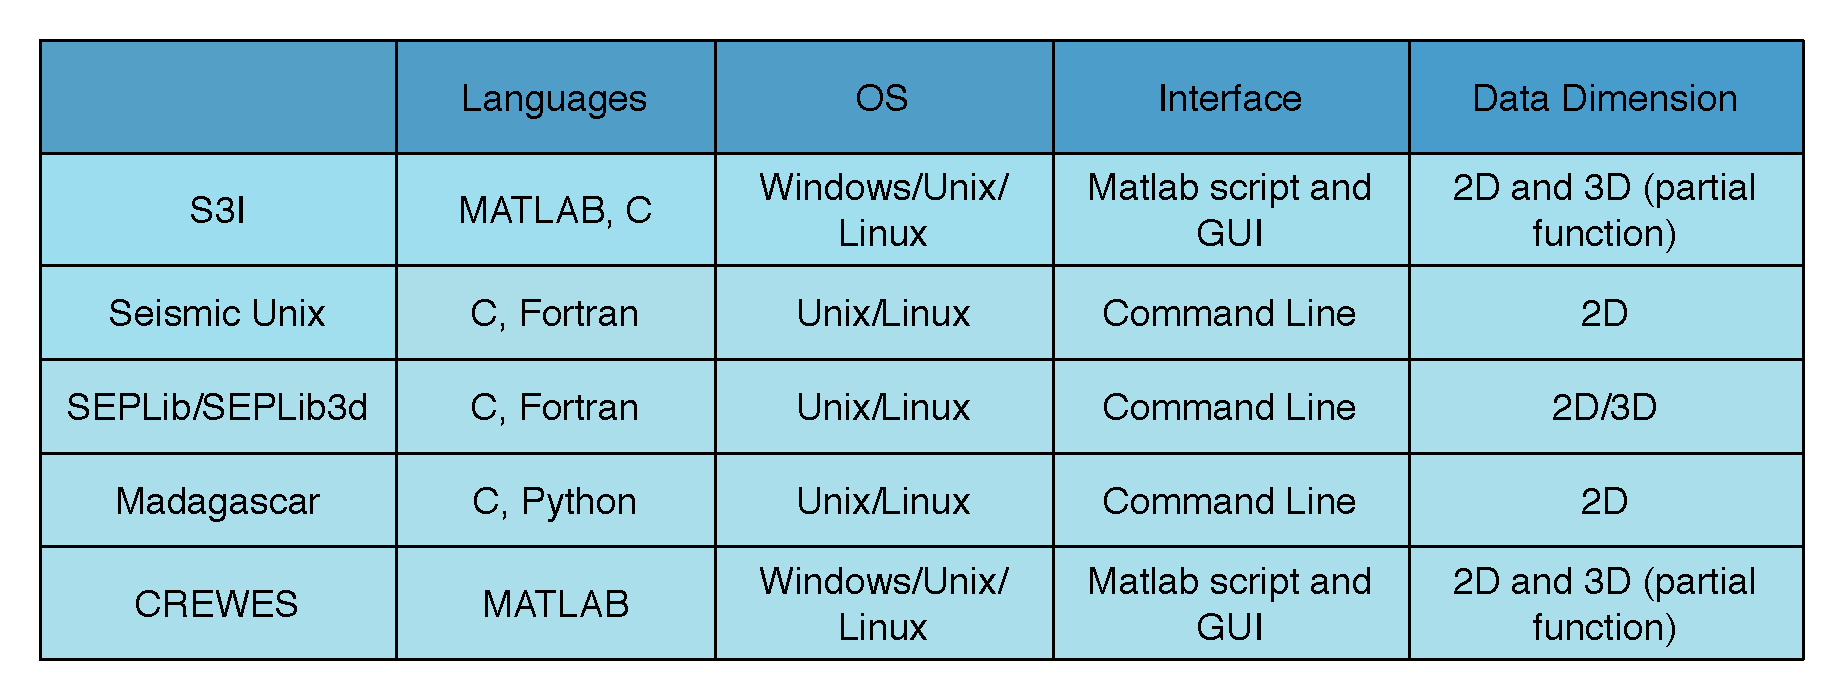
\includegraphics[width=0.9\textwidth]{Fig/comp.eps}
\caption{Comparison of S3I with other open source packages}
\label{fig:comp}
\end{figure}



\section{List of Source Code}
The appendix provides a list of source code in \path{./src} and briefly explains their uses. 

\noindent D\\
\path{dampPml.m}~~~Generates the model for damping parameter for PML\\
\path{dCoef.m}~~~Computes the coefficients of the finite difference using staggered-grid\\

\noindent E\\
\path{eikonal2d.m}~~~Computes the travel time by solving the Eikonal equation in 2-D rectangular domain for a single source\\
\path{extBoundary.m}~~~Performs the zero padding around the given 2-D or 3-D model\\

\noindent F\\
\path{./fd_cmex}~~~source files in C language for finite difference. Run \path{make.m} to compile MEX-files for current system architecture\\
\path{./fd_matlab}~~~source files in Matlab for finite difference, which is not used but only a reference in default\\
\path{fctForAw.m}~~~Performs the FCT method to alleviate numerical grid dispersion for acoustic wave\\
\path{fctForEw.m}~~~Performs the FCT method to alleviate numerical grid dispersion for elastic wave\\
\path{freqFor2dAw.m}~~~Solves the 2-D acoustic wave equation in frequency domain with Enguist-Majda absorbing boundary conditions\\
\path{freqCpmlFor2dAw.m}~~~Solves the 2-D acoustic wave equation in frequency domain with Nonsplit Convolutional-PML\\
\path{fwdTimeCpmlFor3dAw.m}~~~Simulates 3-D acoustic wave forward propagation in time domain with Convolutional-PML\\
\path{fwdTimeSpmlFor2dEw.m}~~~Simulates 2-D elastic wave forward propagation in time domain with Split-PML\\
\path{fwdTimeSpongeFor2dAw.m}~~~Simulates 2-D acoustic wave forward propagation in time domain with sponge absorbing boundary conditions\\

\noindent L\\
\path{layerModelCenerator.m}~~~Generates 2-D or 3-D layered model\\

\noindent M\\
\path{migrate.m}~~~Migrates a shot record for a given travel time between source and receiver using a Kirchoff migration algorithm\\
\path{misfitFuncModel.m}~~~Calculate the least-square misfit function with respect to the perturbation model $\delta \bm$. Used in FWI\\

\noindent P\\
\path{./PQN}~~~the Projected Quasi-Newton (PQN) package for optimization (thanks to Mark Schmidt, Ewout van den Berg, Michael Friedlander, Kevin Murphy from University of British Columbia, Canada)\\
\path{plotTrace.m}~~~Plots seismic traces with filled wiggles\\

\noindent R\\
\path{ray2d.m}~~~Computes the travel time for 2-D model and single point source\\
\path{ricker.m}~~~Generates Ricker wavelet for the source time function\\
\path{rvsTimeSpongeFor2dAw.m}~~~Simulates wave propagation in reverse time with sponge absorbing boundary conditions\\

\noindent S\\
\path{seismic.m}~~~Defines the color space for plotting seismic data\\
\path{shot2RecTime.m}~~~Computes the travel time from a source to a receiver for given travel time map\\

\noindent W\\
\path{waveletGenerator.m}~~~Generates different wavelet as candidates of the source time function\\
\path{wiggle.m}~~~displays seismic data as wiggle plus filled lobes\\

%\noindent S\\
%\path{Seg2FileReader.m}~~~Reads SEG2 files\\
%\path{SegYFileReader.m}~~~Reads SEGY files\\


% References
\bibliographystyle{ieeetr}
\bibliography{UserGuide}


\end{document}
% EOF